%!TEX program = lualatex
%!TEX encoding = UTF-8 Unicode  
%!TEX root = chapter03.tex  
\documentclass[main.tex]{subfiles} 
\begin{document} 
%----------------------------------------------------------------------------------------
%	CHAPTER 1
%----------------------------------------------------------------------------------------
\cleardoublepage 
\loadgeometry{marginlayout}  
\pagestyle{scrheadings} % Print headers again  
\KOMAoptions{
	headwidth=textwithmarginpar,
	headsepline=true,
	headsepline= 0.5pt,
	footwidth=textwithmarginpar,
}   
\onehalfspacing 
\setcounter{chapter}{2}

%----------------------------------------------------------------------------------------
%	 
%----------------------------------------------------------------------------------------
\chapter{Équations du premier degré et systèmes d'équations}




\section{Vocabulaire}
Une \textbf{équation à une inconnue} est une égalité dans laquelle apparaît une ou plusieurs lettres.

\textbf{Une solution} de l’équation est une valeur de la ou les inconnues pour lesquelles l’égalité est vraie. 
\begin{example}\hfill \\
	Soit l'équation $2x+3=x-5$ d'inconnue $x$.
	\begin{enumerate}[label=\alph*),leftmargin=*]
		\item $x=0$ n'est pas solution de l'équation car l'égalité $2\times 0+3=0-5$ est fausse
		\item $x=-8$ est une solution de l'équation, car $2\times(-8)+3=(-8)-5$ est vraie.
	\end{enumerate}
\end{example}
\begin{example}\hfill \\
	Soit l'équation $2x+3y=15$ d'inconnues $x$ et $y$.
	\begin{enumerate}[label=\alph*),leftmargin=*]
		\item Le couple  $x=6$ et $y=1$  est un couple solution car $2\times 6+3\times 1=15$.
%		\item Le couple  $x=-3$ et $y=7$  est un couple solution car $2\times (-3)+3\times 7=15$.
		\item Le couple $x=1$ et $y=6$ n'est pas un couple solution car $2\times 1+3\times 6\neq 15$.  
	\end{enumerate}
\end{example}
\begin{definition} Résoudre une équation dans $\mathbb{R}$ c'est trouver toutes les valeurs  réelles des  inconnues qui rendent l'égalité vraie.
	
	On parle de résolution dans   $\mathbb{N}$ si on cherche uniquement les valeurs entières.
\end{definition} 
\newpage 
\begin{example}\hfill
	\begin{enumerate}[label=\alph*),leftmargin=*]
		\item L'équation $3x=1$ inconnue $x$ n'admet pas de solutions entières.
%		\item L'équation $x^2+1=0$ inconnue $x$, n'admet pas de solutions dans $\mathbb{R}$.
		\item L'équation $x^2-2y^2=0$ d'inconnues $x$ et $y$ n'admet pas de solutions entières.
		\item $x=3$ et $y=2$ est un couple d'entiers solution de l'équation $x^2-2y^2=1$ d'inconnues $x$ et $y$.
	\end{enumerate}
\end{example}

\begin{definition}
	Deux équations sont dites \textbf{équivalentes} (symbole $\iff$) si elles ont le même ensemble de solutions c.à.d elles sont vraies pour les mêmes valeurs de $x$.
\end{definition} 
\begin{example}\hfill 
	\begin{enumerate}[label=\alph*),leftmargin=*]
		\item L'équations $x^2=x$ d'inconnue $x$ a pour solutions $x=0$ et $1$.\\
		L'équation $2x=x+1$ d'inconnue $x$ a une solution unique $x=1$.\\
		Les équations ne sont pas équivalentes.
		\item Les équations $2x=x+1$ et $4x=x+3$ d'inconnues $x$ ont pour seule solution  $x=1$. Elles sont équivalentes.
	\end{enumerate}
\end{example}
%\begin{example} Je vais démontrer que $1=2$.
%	
%	Soit deux nombres non nuls tels que  $a=b$ :
%	
%	$\begin{WithArrows}
%		a& =b \Arrow{$\times a$}\\
%		a^2&=ab\Arrow{$-b^2$}\\
%		a^2-b^2&=ab-b^2\Arrow{on factorise les 2 membres}\\
%		(a-b)(a+b)&=b(a-b)\Arrow{on divise les 2 membres par $(a-b)$}\\
%		a+b&=b \Arrow{par hypotèse $a=b$  }\\
%		2b & = b\Arrow{divise les 2 membres par $b$} \\
%		1& =2
%	\end{WithArrows}$
%\end{example}

%On considère la résolution suivante :  
%\begin{theorem}\label{thm:equaequivalentes} \hfill 
%	
%	$A$, $B$ et $C$ désignent des expressions qui peuvent dépendre d'une inconnue $x$. 
%	\begin{enumerate}
	%		\item  Les équations $A=B$ et $A+C=B+C$ sont équivalentes. 
	%		\item  À condition que $C\neq 0$, les équations $A=B$ et $A \times C =B  \times C$ sont équivalentes.  
	%	\end{enumerate} 
%\end{theorem}
%\begin{proof}\hfill 
%	
%	\vfill 
%\end{proof}

%\begin{exercise}[erreur à éviter]  \hfill 
%	\begin{DispWithArrows*}
	%		(x-3) (x-1)  & =5(x-1)  \Arrow{$\divisionsymbol (x-1)$}\\
	%		(x-3) & = 5  \Arrow{$+ 3$}\\
	%		x & =8  
	%	\end{DispWithArrows*} 
%	Les équations $(x-3) (x-1)  =5(x-1)$ et $x=8$ sont équivalentes. L'ensemble des solutions est $\mathcal{S}=\{8\}$.
%\end{exercise}
 
%----------------------------------------------------------------------------------------
%	 
%----------------------------------------------------------------------------------------



%----------------------------------------------------------------------------------------
%	EXERCICES
%----------------------------------------------------------------------------------------

\newpage 
\loadgeometry{widelayout}  
\pagestyle{scrheadings} % Print headers again  
\KOMAoptions{
	headwidth=textwithmarginpar,
	headsepline=true,
	headsepline= 0.5pt,
	footwidth=textwithmarginpar,
} 
\onehalfspacing
\subsection{Exercices résolution d'équations en isolant l'inconnue}
\begin{exercise}[Vérifier si une valeur est solution d'une équation à 1 inconnue]\hfill 
	
	\noindent\QCM[VF,Alterne,Stretch=1.0, Largeur=0.75cm]{%
%		{$70$ est solution de l'équation $x^{300}=1$ d'inconnue $x$}&2,%
		{$2$ est une solution de l'équation $2x+1=5$ d'inconnue $x$}&1,%
		{$2$ est la solution de l'équation $2x+1=5$ d'inconnue $x$}&1,%
		{$3$ est une solution de l'équation $x^2=3x$ d'inconnue $x$}&1,%
		{$3$ est la solution de l'équation $x^2=3x$ d'inconnue $x$}&2,%
%		{$3$ est une solution de l'équation $\abs{x-5}=2$ inconnue $x$}&1,%
%		{$-3$ est une solution de l'équation $\abs{x-5}=2$ inconnue $x$}&2,%
%		{$-\sqrt{3}$ est une solution de l'équation $3x^2=-9$ inconnue $x$}&2,%
%		{$-\sqrt{3}$ est une solution de l'équation $x^2+2=5$ inconnue $x$}&1,%
%		%	{$\sqrt{3}$ est une solution de l'équation $(3x-1)(x-\sqrt{3})=0$ inconnue $x$}&1,%
%		{$\sqrt{3}$ est une solution de l'équation $(2-x)(2+x)=1$ inconnue $x$}&1,% 
	} 
\end{exercise}
%\vfill 
\begin{exercise}[Vérifier si un couple est solution d'une équation à 2 inconnues]\hfill 
	
	\noindent\QCM[VF,Alterne,Stretch=1.0, Largeur=0.75cm]{%
		{$x=-3$  et $y=3$ est couple solution de l'équation $6x+3y=-2$ d'inconnue  $(x;y)$}&2,%
%		{$x=-\tfrac{2}{3}$  et $y=\tfrac{2}{3}$ est couple solution de l'équation $6x+3y=-2$ d'inconnue  $(x;y)$}&1,% 
		{$x=0$  et $y=-1$ est couple solution de l'équation $-9x-7y=-7$ d'inconnue  $(x;y)$}&2,% 
%		{$x=\tfrac{7}{9}$  et $y=0$ est couple solution de l'équation $-9x-7y=-7$ d'inconnue  $(x;y)$}&1,% 
%		{$x=18$  et $y=\tfrac{323}{20}$ est couple solution de $17x-20y=-17$ d'inconnue  $(x;y)$}&1,% 
		{$x=2$  et $y=5$ est un couple solution de $(x-2)(y+5)=0$ d'inconnue  $(x;y)$}&1,%
		{$x=3$  et $y=-5$ est un couple solution de  $(x-2)(y+5)=0$ d'inconnue  $(x;y)$}&1,% 
		{$x=3$  et $y=\tfrac{1}{3}$ est un couple solution de l'équation $xy=1$ d'inconnue  $(x;y)$}&2,% 
%		{$x=0$  et $y=0$ est le couple solution de l'équation $xy=0$ d'inconnue  $(x;y)$}&2,% 
%		{$x=-6$  et $y=8$ est un couple solution de $x^2+y^2=10^2$ d'inconnue  $(x;y)$}&1,% 
	} 
\end{exercise}

\begin{example} Complétez les espace pour avoir des équations équivalentes d'inconnue $x\in\mathbb{R}$.
	
\tikzset{
%	%Define standard arrow tip
%	>=stealth',
	%Define style for boxes
	point/.style={
		rectangle,
		rounded corners,
		draw=black, very thick,
		text width=6.5em,
		minimum height=2em,
		text centered},
	% Define arrow style
	lien/.style={
		-,
		thick,
		shorten <=0pt,
		shorten >=0pt,},
	lieno/.style={
		-,
		thick,
		shorten <=-2pt,
		shorten >=-2pt,}
}
\noindent
\begin{tikzpicture}[]
	\node [point] (A) at (0,0) {$4x+3=15$};
	\node[point, right=2em of A] (B) {$3=\ldots -4x$}
	(A.east) edge[lien] (B.west) ;
	\node[point, left=2em of A] (F) {$4x-3=\ldots$}
	(A.west) edge[lien] (F.east) ; 
	\node[point, above=1em of A] (D) {$4x=\ldots$}
	(A.north) edge[lien] (D.south) ; 
	\node[point, below=1em of A] (E) {$2x+\numprint{1.5}=\ldots$}
	(A.south) edge[lien] (E.north) ;
	
	\node[point, above=1em of B] (C1) {$8x+6=\ldots$}
	(A.north east) edge[lieno] (C1.south west) ;
	\node[point, below=1em of B] (C2) {$x+\numprint{0.75}=\ldots$}
	(A.south east) edge[lieno] (C2.north west) ;
	
	\node[point, above=1em of F] (C3) {$12x+9=\ldots$}
	(A.north west) edge[lieno] (C3.south east) ;
	\node[point, below=1em of F] (C4) {$x=\ldots$}
	(A.south west) edge[lieno] (C4.north east) ;	 
\end{tikzpicture} 
\end{example}
\begin{exercise} Mêmes consignes, $x$ et $y\in\mathbb{R}$.\hfill 

\noindent
\begin{tikzpicture}[
		%Define style for boxes
	point/.style={
		rectangle,
		rounded corners,
		draw=black, very thick,
		text width=7.5em,
		minimum height=2.2em,
		text centered},
	% Define arrow style
	lien/.style={
		-,
		thick,
		shorten <=0pt,
		shorten >=0pt,},
	lieno/.style={
		-,
		thick,
		shorten <=-2pt,
		shorten >=-2pt,}
	]
	\node [point] (A) at (0,0) {$3x-2=10$};
	\node[point, right=2em of A] (B) {$3x=\ldots $}
	(A.east) edge[lien] (B.west) ;
	\node[point, left=2em of A] (F) {$12-\ldots x=-60$}
	(A.west) edge[lien] (F.east) ; 
	\node[point, above=1em of A] (D) {$\ldots -3x=-10$}
	(A.north) edge[lien] (D.south) ; 
	\node[point, below=1em of A] (E) {$x=\ldots$}
	(A.south) edge[lien] (E.north) ;
	
	\node[point, above=1em of B] (C1) {$\ldots=10=3x$}
	(A.north east) edge[lieno] (C1.south west) ;
	\node[point, below=1em of B] (C2) {$6x-\ldots =20$}
	(A.south east) edge[lieno] (C2.north west) ;
	
	\node[point, above=1em of F] (C3) {$\ldots x -8=40$}
	(A.north west) edge[lieno] (C3.south east) ;
	\node[point, below=1em of F] (C4) {$3x+2=\ldots$}
	(A.south west) edge[lieno] (C4.north east) ;	 
\end{tikzpicture} 

\noindent
\begin{tikzpicture}[
	%Define style for boxes
	point/.style={
		rectangle,
		rounded corners,
		draw=black, very thick,
		text width=7.5em,
		minimum height=2.2em,
		text centered},
	% Define arrow style
	lien/.style={
		-,
		thick,
		shorten <=0pt,
		shorten >=0pt,},
	lieno/.style={
		-,
		thick,
		shorten <=-2pt,
		shorten >=-2pt,}
	]
	\node [point] (A) at (0,0) {$5-2x=25$};
	\node[point, right=2em of A] (B) {$\ldots -4x=50$}
	(A.east) edge[lien] (B.west) ;
	\node[point, left=2em of A] (F) {$\ldots x -15=-75$}
	(A.west) edge[lien] (F.east) ; 
	\node[point, above=1em of A] (D) {$-2x=\ldots$}
	(A.north) edge[lien] (D.south) ; 
	\node[point, below=1em of A] (E) {$\ldots =10-2x$}
	(A.south) edge[lien] (E.north) ;
	
	\node[point, above=1em of B] (C1) {$\ldots +2x=5$}
	(A.north east) edge[lieno] (C1.south west) ;
	\node[point, below=1em of B] (C2) {$x=\ldots$}
	(A.south east) edge[lieno] (C2.north west) ;
	
	\node[point, above=1em of F] (C3) {$\numprint{2.5}-x=\ldots$}
	(A.north west) edge[lieno] (C3.south east) ;
	\node[point, below=1em of F] (C4) {$\ldots -8x=100$}
	(A.south west) edge[lieno] (C4.north east) ;	 
\end{tikzpicture} 


\noindent\begin{tikzpicture}[
	%Define style for boxes
	point/.style={
		rectangle,
		rounded corners,
		draw=black, very thick,
		text width=7.5em,
		minimum height=2.2em,
		text centered},
	% Define arrow style
	lien/.style={
		-,
		thick,
		shorten <=0pt,
		shorten >=0pt,},
	lieno/.style={
		-,
		thick,
		shorten <=-2pt,
		shorten >=-2pt,}
	]
	\node [point] (A) at (0,0) {$4x+3y=15$};
	\node[point, right=2em of A] (B) {$4x=15-\ldots y$}
	(A.east) edge[lien] (B.west) ;
	\node[point, left=2em of A] (F) {$3y=\ldots -4x$}
	(A.west) edge[lien] (F.east) ; 
	\node[point, above=1em of A] (D) {$60=\ldots x +12y$}
	(A.north) edge[lien] (D.south) ; 
	\node[point, below=1em of A] (E) {$\ldots x +\ldots y=45$}
	(A.south) edge[lien] (E.north) ;
	
	\node[point, above=1em of B] (C1) {$15y=\ldots -20x$}
	(A.north east) edge[lieno] (C1.south west) ;
	\node[point, below=1em of B] (C2) {$x+\ldots y=\numprint{3.75}$}
	(A.south east) edge[lieno] (C2.north west) ;
	
	\node[point, above=1em of F] (C3) {$8x+6y=\ldots$}
	(A.north west) edge[lieno] (C3.south east) ;
	\node[point, below=1em of F] (C4) {$\numprint{0.4}x+\ldots y=\ldots$}
	(A.south west) edge[lieno] (C4.north east) ;	 
\end{tikzpicture} 
\end{exercise}
%\vfill 
\begin{tBox}
	On ne change pas les solutions d'une équation si :
	\begin{enumerate}[label=\textbullet, leftmargin=*]
		\item on \textbf{additionne, soustrait} aux \textbf{2 membres} de l'équation  une même expression.
		\item on \textbf{multiplie/divise} les \textbf{2 membres} de l'équation par \textbf{une même}  expression \textbf{non nulle}.
		\item on \textbf{développe, factorise, réduit ...} un des deux membres de l'équation.
	\end{enumerate}  
\end{tBox} 
\begin{example}  Résoudre dans $\mathbb{R}$ les équations suivantes d'inconnue $x$ :\hfill 
	
	\noindent \parbox{0.23\linewidth}{	
		$\begin{WithArrows}
			7x&=-25 \\
			&  \rule{0pt}{1.3em}   \\
			&  \rule{0pt}{1.3em}   \\
			&  \rule{0pt}{1.3em}    
		\end{WithArrows}$ 	
	}\hfill \parbox{0.23\linewidth}{	
		$\begin{WithArrows}
			-\frac{3}{4}x&=13 \\
			&  \rule{0pt}{1.3em}   \\
			&  \rule{0pt}{1.3em}   \\
			&  \rule{0pt}{1.3em}   
		\end{WithArrows}$ 
	} \hfill \parbox{0.23\linewidth}{	
		$\begin{WithArrows}
			-3x-9&=0 \\
			&  \rule{0pt}{1.3em}   \\
			&  \rule{0pt}{1.3em}   \\
			&  \rule{0pt}{1.3em}   
		\end{WithArrows}$ 
	}  \hfill \parbox{0.23\linewidth}{	
		$\begin{WithArrows}
			\frac{2}{3}x-\frac{1}{4}&=\frac{5}{6} \\
			&  \rule{0pt}{1.3em}   \\
			&  \rule{0pt}{1.3em}   \\
			&  \rule{0pt}{1.3em}    
		\end{WithArrows}$ 
	}   
\end{example}
\begin{exercise}[résoudre en 1 étape]\label{chapter07:exercice:equation01} Même consignes
	\vspace{-1em} 
	
	\begin{multicols}{5}
		\begin{enumerate}[label={$(E_{\arabic*})$}, leftmargin=*]
			\item $6x=-42$
			\item $24x=-8$
			\item $-\tfrac{3}{5}x=-60$
			\item $\tfrac{x}{6}=12$
			\item $\tfrac{x}{9}=-18$
			\item $-x=100$
			\item $24=\tfrac{x}{3}$
			\item $\tfrac{3}{4}x=24$
			\item $42x=0$
			\item $-\tfrac{5}{3}x=12$ 
		\end{enumerate}
	\end{multicols}  
\end{exercise}
\vspace{-1em} 

\begin{exercise}[résoudre en 2 étapes]\label{chapter07:exercice:equation02}  Mêmes consignes \hfill 
	\vspace{-1em} 
	\begin{multicols}{4}
		\begin{enumerate}[label={$(E_{\arabic*})$}, leftmargin=*]
			\item $4x-9=0$
			\item $-10=3x+7$
			\item $-81=-51-3x$
			\item $\tfrac{2}{7}x -5=12$
			\item $-\tfrac{2}{9}x+\tfrac{5}{3}=-2$ 
			\item $-\tfrac{4}{3}x-\tfrac{5}{3}=\tfrac{1}{6}$ 
			\item $-\tfrac{7}{9}x-\tfrac{6}{7}=\tfrac{31}{21}$
			\item $\tfrac{9}{7}x+\tfrac{2}{3}=\tfrac{17}{21}$
		\end{enumerate}
	\end{multicols}  
\end{exercise}
\vspace{-1em}
%\newpage  
\begin{example}  Résoudre dans $\mathbb{R}$ les équations suivantes d'inconnue $x$ :\hfill 
	
	\noindent \parbox{0.33\linewidth}{	
		$\begin{WithArrows}
			4(x+1)&=x+7   
		\end{WithArrows}$ 	
	}\hfill \parbox{0.33\linewidth}{	
		$\begin{WithArrows}
			4(x-1)&=-7x+5 
		\end{WithArrows}$ 
}\hfill \parbox{0.33\linewidth}{	
$\begin{WithArrows}
	-2(3x-6)&=3(-2x+4)    
\end{WithArrows}$ 
} 
\vfill    
\end{example} 
%\newpage 
\begin{exercise}\label{chapter07:exercice:equationA} Résoudre dans $\mathbb{R}$ les équations suivantes d'inconnue $x$: \hfill 
	\vspace{-1em}
	\begin{multicols}{3}
		\begin{enumerate}[label={$(E_{\arabic*})$}, leftmargin=*]
			\item $3(x+5)=x+1$
			\item $3(x+5)=3(2x+1)$
			\item $3(x+5)-3(2x-1)=0$
			\item $3(2x-5)=3(x-1)$
			\item $3(x-5)=-3(2x+1)$ 
			\item $-3(2x+5)=-3(2x+1)$
			\item $2(3x-6)-3(-2x+4)=5$
			\item $-3(x-5)=4-3(2x-1)$
			\item $-3(2x-1)=x-3(x-5)$ 
			%		\item[$E_{1}\colon $] $x+5=3(x+1)$   
			%		\item[$E_{7}\colon$]  $ 3(x-5)=3(2x+1)$
		\end{enumerate}
	\end{multicols} 	
\end{exercise}
\vspace{-1em}  
\begin{example}  Résoudre dans $\mathbb{R}$ les équations suivantes d'inconnue $x$: 
	
	\noindent \parbox{0.45\linewidth}{	
		$\begin{WithArrows}
			\tfrac{x+1}{4}+\tfrac{5}{6}&=\tfrac{9}{2}   
		\end{WithArrows}$ 	
	}\hfill \parbox{0.45\linewidth}{	
		$\begin{WithArrows}
			\tfrac{x+2}{2}-\tfrac{x-4}{6}&=6 
		\end{WithArrows}$ 
	}   
\end{example}
%\newpage
\vfill 
\begin{exercise}\label{chapter07:exercice:equationB} Résoudre dans $\mathbb{R}$ les équations suivantes d'inconnue $x$: \hfill
	  \vspace{-1em}
	\begin{multicols}{4}
		\begin{enumerate}[label={$(E_{\arabic*})$\rule{0pt}{2em}}, leftmargin=*]
%			\item $\frac{x}{6}+\frac{x}{4}=\frac{5}{6}$
			\item $\frac{x}{3}-\frac{x}{4}=-\frac{5}{4}$
			\item $\frac{x}{2}-\frac{x+5}{3}=\frac{1}{2}$
%			\item $\frac{3x}{5}-\frac{x}{4}=\frac{1}{20}$
			\item $\frac{3x}{5}-\frac{x+2}{4}=0$ 
%			\item $\frac{x}{4}+\frac{x}{12}=\frac{1}{6}$ 
			\item  $\frac{x+2}{6}+\frac{x+4}{8}=9$
%			\item  $\frac{2x-1}{3}-\frac{x}{2}=3x$
%			\item $\frac{x}{2}=1+\frac{2x-1}{3}$
		\end{enumerate}
	\end{multicols} 	
\end{exercise}

%\begin{exercise}\label{chapter07:exercice:equationB} Résoudre dans $\mathbb{R}$ les équations suivantes d'inconnue $x$: \hfill  
%	\begin{multicols}{3}
	% 		\begin{enumerate}[label={$(E_{\arabic*})$}, leftmargin=*]
		% 			\item $\tfrac{1}{4}x+\tfrac{22}{45}=0$
		% 			\item $\tfrac{2}{3}x-\tfrac{22}{15}=0$
		% 			\item $\tfrac{4}{3}x+1=0$
		%			\item $	\tfrac{x+2}{2}+\tfrac{x+4}{3}=4$
		%			\item $	\tfrac{x+2}{2}+\tfrac{x+4}{8}=4x$
		%			\item $	\tfrac{x+2}{6}+\tfrac{x+4}{8}=9$
		%			\item $ \tfrac{x+2}{6}-\tfrac{x+4}{8}=9$
		%			\item $	\tfrac{x-2}{6}-\tfrac{x-4}{8}=9$
		%			\item $\tfrac{2x-1}{3}-\tfrac{x}{2}=3x$
		%			\item $	\tfrac{4x-4}{8}-\tfrac{4x-2}{6}=9$
		%			\item $\tfrac{x}{2}-\tfrac{2x-1}{3}=1$
		%			\item $\tfrac{x-5}{3}-2(x-7)=2x+1$
		%			%			\item[$E_{3}\colon$]  $	\frac{x+2}{2}+\frac{x+4}{8}=9$
		%			%			\item[$E_{6}\colon$] $ \frac{x+2}{6}-\frac{x-4}{8}=9$ 
		%			%			\item[$E_{8}\colon$] $\frac{2x-2}{2}-\frac{2x-4}{8}=9$
		%			%			\item[$E_{11}\colon$] $	\frac{4x-4}{8}-\frac{4x-2}{6}=1$
		%		\end{enumerate}
	%	\end{multicols} 	
%\end{exercise}
%----------------------------------------------------------------------------------------
%	 
%----------------------------------------------------------------------------------------
\newpage 
%\section{Exercices isoler l'inconnue pour résoudre}
%\begin{example} Résoudre dans $\mathbb{R}$ les équations suivantes d'inconnue $x$.
%	
%	\noindent \parbox{0.20\linewidth}{	
%		$\begin{WithArrows}
%			\abs{x}&=  10 \\ 
%			& \rule{0pt}{1.3em}  \\
%			&  \rule{0pt}{1.3em} \\
%			&   \rule{0pt}{1.3em}  
%		\end{WithArrows}$ 	
%	}\hfill \parbox{0.20\linewidth}{	
%		$\begin{WithArrows}
%			2\abs{x}-5&=  10 \\ 
%			& \rule{0pt}{1.3em}  \\
%			&  \rule{0pt}{1.3em} \\
%			&   \rule{0pt}{1.3em}  
%		\end{WithArrows}$ 	
%	}\hfill \parbox{0.20\linewidth}{	
%		$\begin{WithArrows}
%			\abs{2x-5}&=  10 \\ 
%			& \rule{0pt}{1.3em}  \\
%			&  \rule{0pt}{1.3em} \\
%			&   \rule{0pt}{1.3em}  
%		\end{WithArrows}$ 	
%	}\hfill \parbox{0.30\linewidth}{	
%		$\begin{WithArrows}
%			\abs{2x-7}&=\abs{x+3} \\ 
%			& \rule{0pt}{1.3em}  \\
%			&  \rule{0pt}{1.3em} \\
%			&   \rule{0pt}{1.3em}  
%		\end{WithArrows}$ 	
%	} 
%\end{example}
%\vfill 
%\begin{exercise}\label{chapter07:exercice:equationC} Résoudre dans $\mathbb{R}$ les équations suivantes d'inconnue $x$: \hfill  
%	\begin{multicols}{3}
%		\begin{enumerate}[label={$(E_{\arabic*})$}, leftmargin=*]
%			\item  $\abs{2x}=3$
%			\item  $3\abs{x} + 5=14$
%			\item  $3\abs{x} + 5=4$
%			\item  $\abs{3x-5}=7$
%			\item  $\abs{4x-3}=-1$ 
%			\item  $5\abs{x}-3=6$
%			\item  $-2\abs{x}+11=6$  
%			\item  $-3\abs{x}+2=6$
%			\item  $\abs{5-2x}=10^{-2}$
%			\item  $\abs{3x+1}=\abs{x}$
%			\item  $\abs{2x-1}=\abs{2x-7}$
%			\item  $\abs{5x+1}=\abs{2x+5}$
%		\end{enumerate}
%	\end{multicols} 	
%\end{exercise}

 
\begin{example}[équation et angles]Les flèches indiquent des droites parallèles, et les segments qui semblent alignés le sont. 
	Écrire une équation en $x$ et la résoudre. 
	
	\noindent
	\parbox{0.23\linewidth}{
		\begin{tikzpicture}[scale=0.9] 
			\tkzSetUpPoint[size=3, fill=black]
			\tkzfctset{tan style/.style={->,>=latex, color=red, line width=1.2pt}}   
			\tkzSetUpLine[line width= 1.2pt, add=.5 and .5] 
			
			\def\xa{0}
			\def\xb{60}
			\def\xc{180}
			\def\xd{240}
			\def\Rayon{2.5}
			\def\rayon{2.0}
			\tkzDefPoints{0/0/O}
			\tkzDefShiftPoint[O](\xa:\rayon){A}
			\tkzDefShiftPoint[O](\xb:\Rayon){B}
			\tkzDefShiftPoint[O](\xc:\rayon){C}
			\tkzDefShiftPoint[O](\xd:\Rayon){D}
			\tkzDrawSegments[line width=1.2pt](A,C B,D)
			
			\tkzMarkAngle[mark=none,-,size=0.65](B,O,C)
			\tkzFillAngle[opacity=.5,size=0.65](B,O,C)
			\tkzLabelAngle[pos=1.0](B,O,C){$\ang{115}$}
			\tkzMarkAngle[mark=none,-,size=0.65](C,O,D)
			\tkzFillAngle[opacity=.5,size=0.65](C,O,D)
			\tkzLabelAngle[pos=1.25](C,O,D){$5x$} 
		\end{tikzpicture} 
	}\hfill   
	\parbox{0.23\linewidth}{ 
		$\begin{WithArrows}
			5x+115&=180\\
			-115 & \; -115\\
			5x&=65\\
			\frac{5x}{5}&=\frac{65}{5}\\
			x&=13
		\end{WithArrows}$
	}	 \hfill
	\parbox{0.28\linewidth}{
		\begin{tikzpicture}[scale=1.0] 
			\tkzSetUpPoint[size=3, fill=black]
			\tkzfctset{tan style/.style={->,>=latex, color=red, line width=1.2pt}}   
			\tkzSetUpLine[line width= 1.2pt, add=.2 and .2] 
			
			\def\taille{0.5}
			\def\xa{-20}
			\def\xb{60}
			\def\xc{180}
			\def\xd{240}
			\def\Rayon{2.5}
			\def\rayon{2.0}
			\tkzDefPoints{0/0/O1,-0.3/2.5/O2}
			
			\tkzDefShiftPoint[O1](\xa:\rayon){A}
			\tkzDefShiftPoint[O1]({\xa+180}:\rayon){B}
			\tkzDefShiftPoint[O2](\xa:\rayon){C}
			\tkzDefShiftPoint[O2]({\xa+180}:1.5){D}
			\tkzDrawSegments[line width=1.2pt](A,B C,D)
			\tkzMarkSegments[mark=none, tkz arrow={Stealth[scale=2]  at 0.8 }](O1,A O2,C)
			\tkzDrawLine(O1,O2)
			
			\tkzMarkAngle[mark=none,-,size=\taille](A,O1,O2)
			\tkzFillAngle[opacity=.5,size=\taille](A,O1,O2)
			\tkzLabelAngle[pos=1.0](A,O1,O2){$\ang{100}$}
			\tkzMarkAngle[mark=none,-,size=\taille](O1,O2,C)
			\tkzFillAngle[opacity=.5,size=\taille](O1,O2,C)
			\tkzLabelAngle[pos=1.0](O1,O2,C){$5x$} 
		\end{tikzpicture}	
	}\hfill 
	\parbox{0.23\linewidth}{  
		$\begin{WithArrows}
			5x+100&=180\\
			-100 & \; -100\\ 
			5x&=80\\
			\frac{5x}{5}&=\frac{80}{5}\\
			x&=16
		\end{WithArrows}$
	}	
\end{example}
\begin{exercise}\hfill 

\noindent 
\parbox{0.30\linewidth}{
\begin{tikzpicture}[scale=1.0] 
	\tkzSetUpPoint[size=3, fill=black]
	\tkzfctset{tan style/.style={->,>=latex, color=red, line width=1.2pt}}   
	\tkzSetUpLine[line width= 1.2pt, add=.2 and .2] 
	
	\def\taille{0.65}
	\def\xa{0}
	\def\xb{60}
	\def\xc{180}
	\def\xd{240}
	\def\Rayon{2.5}
	\def\rayon{2.0}
	\tkzDefPoints{0/0/O}
	\tkzDefShiftPoint[O](\xa:\rayon){A}
	\tkzDefShiftPoint[O](\xb:\rayon){B}
	\tkzDefShiftPoint[O](\xc:\rayon){C}
	\tkzDefShiftPoint[O](\xd:\rayon){D}
	\tkzDrawSegments[line width=1.2pt](A,C O,B)
	
	\tkzMarkAngle[mark=none,-,size=\taille](A,O,B)
	\tkzFillAngle[opacity=.5,size=\taille](A,O,B)
	\tkzLabelAngle[pos=1.0](A,O,B){$3x$}
	\tkzMarkAngle[mark=none,-,size=\taille](B,O,C)
	\tkzFillAngle[opacity=.5,size=\taille](B,O,C)
	\tkzLabelAngle[pos=1.25](B,O,C){$\ang{114}$} 
\end{tikzpicture} 
}\hfill 
\parbox{0.30\linewidth}{
\begin{tikzpicture}[scale=1.0] 
	\tkzSetUpPoint[size=3, fill=black]
	\tkzfctset{tan style/.style={->,>=latex, color=red, line width=1.2pt}}   
	\tkzSetUpLine[line width= 1.2pt, add=.5 and .5] 
	
	\def\taille{0.65}
	\def\xa{-40}
	\def\xb{\xa+60}
	\def\xc{\xa+180}
	\def\xd{240}
	\def\Rayon{2.5}
	\def\rayon{2.0}
	\tkzDefPoints{0/0/O}
	\tkzDefShiftPoint[O](\xa:\rayon){A}
	\tkzDefShiftPoint[O](\xb:\rayon){B}
	\tkzDefShiftPoint[O](\xc:\rayon){C}
	\tkzDefShiftPoint[O](\xd:\rayon){D}
	\tkzDrawSegments[line width=1.2pt](A,C O,B)
	
	\tkzMarkAngle[mark=none,-,size=\taille](A,O,B)
	\tkzFillAngle[opacity=.5,size=\taille](A,O,B)
	\tkzLabelAngle[pos=1.0](A,O,B){$4x$}
	\tkzMarkAngle[mark=none,-,size=\taille](B,O,C)
	\tkzFillAngle[opacity=.5,size=\taille](B,O,C)
	\tkzLabelAngle[pos=1.25](B,O,C){$\ang{96}$} 
\end{tikzpicture} 
}  
\hfill 
\parbox{0.30\linewidth}{
\begin{tikzpicture}[scale=1.0] 
	\tkzSetUpPoint[size=3, fill=black]
	\tkzfctset{tan style/.style={->,>=latex, color=red, line width=1.2pt}}   
	\tkzSetUpLine[line width= 1.2pt, add=.5 and .5] 
	
	\def\taille{0.65}
	\def\xa{-150}
	\def\xb{\xa+90}
	\def\xc{\xb+40}
	\def\xd{\xa+180}
	\def\Rayon{2.5}
	\def\rayon{2.0}
	\tkzDefPoints{0/0/O}
	\tkzDefShiftPoint[O](\xa:\rayon){A}
	\tkzDefShiftPoint[O](\xb:\rayon){B}
	\tkzDefShiftPoint[O](\xc:\rayon){C}
	\tkzDefShiftPoint[O](\xd:\rayon){D}
	\tkzDrawSegments[line width=1.2pt](O,A O,B O,C O,D)
	
	\tkzMarkRightAngle[size=\taille](A,O,B)
	\tkzMarkAngle[mark=none,-,size=\taille](B,O,C)
	\tkzFillAngle[opacity=.5,size=\taille](B,O,C)
	\tkzLabelAngle[pos=1.0](B,O,C){$2x$}
	\tkzMarkAngle[mark=none,-,size=\taille](C,O,D)
	\tkzFillAngle[opacity=.5,size=\taille](C,O,D)
	\tkzLabelAngle[pos=1.25](C,O,D){$3x$} 
\end{tikzpicture} 
}  

\vfill 

\noindent
\parbox{0.30\linewidth}{
\begin{tikzpicture}[scale=1.0] 
	\tkzSetUpPoint[size=3, fill=black]
	\tkzfctset{tan style/.style={->,>=latex, color=red, line width=1.2pt}}   
	\tkzSetUpLine[line width= 1.2pt, add=.5 and .5] 
	
	\def\taille{0.65}
	\def\xa{-20}
	\def\xb{185}
	\def\xc{180}
	\def\xd{240}
	\def\Rayon{2.5}
	\def\rayon{2.0}
	\tkzDefPoints{0/0/O}
	\tkzDefShiftPoint[O](\xa:\rayon){A}
	\tkzDefShiftPoint[O](\xb:\rayon){B}
	\tkzDefShiftPoint[O](\xc:\rayon){C}
	\tkzDefShiftPoint[O](\xd:\rayon){D}
	\tkzDrawSegments[line width=1.2pt](O,A O,B)
	
	\tkzMarkAngle[mark=none,-,size=\taille](A,O,B)
	\tkzFillAngle[opacity=.5,size=\taille](A,O,B)
	\tkzLabelAngle[pos=1.0](A,O,B){$\ang{210}$}
	\tkzMarkAngle[mark=none,-,size=\taille](B,O,A)
	\tkzFillAngle[opacity=.5,size=\taille](B,O,A)
	\tkzLabelAngle[pos=1.25](B,O,A){$6x$} 
\end{tikzpicture} 
}   
\hfill
\parbox{0.30\linewidth}{
\begin{tikzpicture}[scale=1.0] 
	\tkzSetUpPoint[size=3, fill=black]
	\tkzfctset{tan style/.style={->,>=latex, color=red, line width=1.2pt}}   
	\tkzSetUpLine[line width= 1.2pt, add=.5 and .5] 
	
	\def\taille{0.65}
	\def\xa{-30}
	\def\xb{\xa+55}
	\def\xc{\xa+180}
	\def\xd{\xb+180}
	\def\Rayon{2.5}
	\def\rayon{2.0}
	\tkzDefPoints{0/0/O}
	\tkzDefShiftPoint[O](\xa:\rayon){A}
	\tkzDefShiftPoint[O](\xb:\rayon){B}
	\tkzDefShiftPoint[O](\xc:\rayon){C}
	\tkzDefShiftPoint[O](\xd:\rayon){D}
	\tkzDrawSegments[line width=1.2pt](O,A O,B O,C O,D)
	
	\tkzMarkAngle[mark=none,-,size=\taille](A,O,B)
	\tkzFillAngle[opacity=.5,size=\taille](A,O,B)
	\tkzLabelAngle[pos=1.0](A,O,B){$\ang{72}$}
	\tkzMarkAngle[mark=none,-,size=\taille](C,O,D)
	\tkzFillAngle[opacity=.5,size=\taille](C,O,D)
	\tkzLabelAngle[pos=1.25](C,O,D){$6x$}  
\end{tikzpicture} 
}   
\hfill 
\parbox{0.28\linewidth}{
\begin{tikzpicture}[scale=1.0] 
	\tkzSetUpPoint[size=3, fill=black]
	\tkzfctset{tan style/.style={->,>=latex, color=red, line width=1.2pt}}   
	\tkzSetUpLine[line width= 1.2pt, add=.2 and .2] 
	
	\def\taille{0.5}
	\def\xa{-20}
	\def\xb{\xa+65}
	\def\xc{180}
	\def\xd{240}
	\def\Rayon{2.0}
	\def\rayon{1.0}
	\tkzDefPoints{0/0/O1}
	\tkzDefShiftPoint[O1](\xa:\Rayon){O2}
	\tkzDefShiftPoint[O2](\xa:\rayon){A}
	\tkzDefShiftPoint[O1](\xb:\Rayon){C}
	\tkzDefShiftPoint[O2](\xb:\Rayon){B} 
	%		\tkzDefShiftPoint[O2]({\xa+180}:\rayon){D}
	\tkzDrawSegments[line width=1.2pt](O1,C O2,B)
	\tkzMarkSegments[mark=none, tkz arrow={Stealth[scale=2]  at 0.7 }](O1,C O2,B)
	\tkzDrawLine(O1,A)
	
	\tkzMarkAngle[mark=none,-,size=\taille](A,O2,B)
	\tkzFillAngle[opacity=.5,size=\taille](A,O2,B)
	\tkzLabelAngle[pos=1.2](A,O2,B){$5x+15$}
	\tkzMarkAngle[mark=none,-,size=\taille](O2,O1,C)
	\tkzFillAngle[opacity=.5,size=\taille](O2,O1,C)
	\tkzLabelAngle[pos=1.0](O2,O1,C){$\ang{55}$} 
\end{tikzpicture}	
}

\vfill 

\noindent
\parbox{0.30\linewidth}{
	\begin{tikzpicture}[scale=1.0] 
		\tkzSetUpPoint[size=3, fill=black]
		\tkzfctset{tan style/.style={->,>=latex, color=red, line width=1.2pt}}   
		\tkzSetUpLine[line width= 1.2pt, add=.5 and .5] 
		
		\def\taille{0.65}
		\def\xa{-15}
		\def\xb{\xa+55}
		\def\xc{\xa+180}
		\def\xd{\xb+180} 
		\def\cote{4.0}
		\tkzDefPoints{0/0/A} 
		\tkzDefShiftPoint[A](\xa:\cote){B}
		
		\tkzDefTriangle[two angles=90 and 30](A,B)\tkzGetPoint{C}
		\tkzDrawPolygon[line width=1.2pt](A,B,C)
		
		\tkzMarkRightAngle[size=0.4](B,A,C)
		\tkzMarkAngle[mark=none,-,size=\taille](C,B,A)
		\tkzFillAngle[opacity=.5,size=\taille](C,B,A)
		\tkzLabelAngle[pos=1.25](C,B,A){$7x$}
		\tkzMarkAngle[mark=none,-,size=\taille](A,C,B)
		\tkzFillAngle[opacity=.5,size=\taille](A,C,B)
		\tkzLabelAngle[pos=1.0](A,C,B){$11x$}  
	\end{tikzpicture} 
}  
\hfill
\parbox{0.25\linewidth}{  
	\begin{tikzpicture}[xscale=1, yscale=1]
		\tkzSetUpPoint[size=4, fill=black]	
		\tkzSetUpLine[line width= 1.2pt, add=.5 and .5] 
		\tkzfctset{tan style/.style={->,>=latex, color=red, line width=1.2pt}} 
	 
		
		\def\a{5}
		\def\b{180+\a-58}
		\def\c{180+\b-140}
		\tkzDefPoints{0/0/A}
		\tkzDefShiftPoint[A]({\a}:4){B}
		\tkzDefShiftPoint[B]({\b}:3){C}
		\tkzDefShiftPoint[C]({\c}:2.2){D}
		\tkzDrawPolygon[line width=1.2pt](A,B,C,D)
		
		\tkzLabelAngle[pos=1.0](B,A,D){$3x$}
		\tkzMarkAngle[mark=none,-,size=0.65](B,A,D)
		\tkzFillAngle[opacity=.5,size=0.65](B,A,D)
		
		
		\tkzLabelAngle[pos=1.0](C,B,A){$\ang{80}$}
		\tkzMarkAngle[mark=none,-,size=0.65](C,B,A)
		\tkzFillAngle[opacity=.5,size=0.65](C,B,A)
		
		
		\tkzLabelAngle[pos=1.0](D,C,B){$2x+40$}
		\tkzMarkAngle[mark=none,-,size=0.65](D,C,B)
		\tkzFillAngle[opacity=.5,size=0.65](D,C,B)
		
		
		\tkzLabelAngle[pos=1.0](A,D,C){$x$}
		\tkzMarkAngle[mark=none,-,size=0.65](A,D,C)
		\tkzFillAngle[opacity=.5,size=0.65](A,D,C)
		
%		\tkzLabelSegment[above right](B,C){$x$} 
	\end{tikzpicture} 
} 
\end{exercise}
 




\begin{exercise}  Pour chaque figure, écrire une équation en $a$  et la résoudre. En déduire que $ABC$ est un triangle rectangle, $DEF$ est un triangle isocèle et $SHIP$ est un parallélogramme.
	
\noindent 
\parbox{0.33\linewidth}{
\begin{tikzpicture}[xscale=1, yscale=1]
	\tkzSetUpPoint[size=4, fill=black]	
	\tkzSetUpLine[line width= 1.2pt, add=.5 and .5] 
	\tkzfctset{tan style/.style={->,>=latex, color=red, line width=1.2pt}} 
	
   
	
	\def\a{-6} 
	\tkzDefPoints{0/0/A}
	\tkzDefShiftPoint[A]({\a}:5){B}
	\tkzDefTriangle[two angles=40 and 60](A,B)\tkzGetPoint{C}
	\tkzDrawPolygon[line width=1.2pt](A,B,C)
	
	\tkzLabelAngle[pos=1.0](B,A,C){$a$}
	\tkzMarkAngle[mark=none,-,size=0.65](B,A,C)
	\tkzFillAngle[opacity=.5,size=0.65](B,A,C)
	
	\tkzLabelAngle[pos=1.2](C,B,A){$2a-\ang{6}$}
	\tkzMarkAngle[mark=none,-,size=0.65](C,B,A)
	\tkzFillAngle[opacity=.5,size=0.65](C,B,A)
	
	\tkzLabelAngle[pos=1.2](A,C,B){$2a+\ang{26}$}
	\tkzMarkAngle[mark=none,-,size=0.65](A,C,B)
	\tkzFillAngle[opacity=.5,size=0.65](A,C,B)
	
%	\tkzLabelSegment[below](A,B){$x$}
%	\tkzLabelSegment[above right](B,C){\SI{10}{\centi\meter}}
%	\tkzLabelSegment[above left](C,A){$y$}
	
	
	\tkzLabelPoint[below](A){$A$}
	\tkzLabelPoint[right](B){$B$}
	\tkzLabelPoint[above](C){$C$}  
\end{tikzpicture}  
}
\parbox{0.33\linewidth}{
	\begin{tikzpicture}[xscale=1, yscale=1]
		\tkzSetUpPoint[size=4, fill=black]	
		\tkzSetUpLine[line width= 1.2pt, add=.5 and .5] 
		\tkzfctset{tan style/.style={->,>=latex, color=red, line width=1.2pt}} 
		
		
		
		\def\a{-5} 
		\tkzDefPoints{0/0/A}
		\tkzDefShiftPoint[A]({\a}:4.5){B}
		\tkzDefTriangle[two angles=55 and 55](A,B)\tkzGetPoint{C}
		\tkzDrawPolygon[line width=1.2pt](A,B,C)
		
		\tkzLabelAngle[pos=1.3](B,A,C){\small$5a-\ang{23}$}
		\tkzMarkAngle[mark=none,-,size=0.65](B,A,C)
		\tkzFillAngle[opacity=.5,size=0.65](B,A,C)
		
		\tkzLabelAngle[pos=1.3](C,B,A){\small$2a+\ang{16}$}
		\tkzMarkAngle[mark=none,-,size=0.65](C,B,A)
		\tkzFillAngle[opacity=.5,size=0.65](C,B,A)
		
		\tkzLabelAngle[pos=1.3](A,C,B){\small$4a+\ang{44}$}
		\tkzMarkAngle[mark=none,-,size=0.65](A,C,B)
		\tkzFillAngle[opacity=.5,size=0.65](A,C,B)
		
		%	\tkzLabelSegment[below](A,B){$x$}
		%	\tkzLabelSegment[above right](B,C){\SI{10}{\centi\meter}}
		%	\tkzLabelSegment[above left](C,A){$y$}
		
		
		\tkzLabelPoint[below](A){$D$}
		\tkzLabelPoint[right](B){$E$}
		\tkzLabelPoint[above](C){$F$}  
	\end{tikzpicture}  
}
\parbox{0.33\linewidth}{ 
	\begin{tikzpicture}[xscale=0.9, yscale=0.9]
		\tkzSetUpPoint[size=4, fill=black]	
		\tkzSetUpLine[line width= 1.2pt, add=.5 and .5] 
		\tkzfctset{tan style/.style={->,>=latex, color=red, line width=1.2pt}} 
	  
			\def\a{-10}
			\def\b{180+\a-71}
			\def\c{180+\b-91}
			\tkzDefPoints{0/0/A}
			\tkzDefShiftPoint[A]({\a}:5){B}
			\tkzDefShiftPoint[B]({\b}:4.5){C}
			\tkzDefShiftPoint[C]({\c}:3.5){D}
			\tkzDrawPolygon[line width=1.2pt](A,B,C,D)
			
			\tkzLabelAngle[pos=1.2](B,A,D){\small$5a-\ang{15}$}
			\tkzMarkAngle[mark=none,-,size=0.65](B,A,D)
			\tkzFillAngle[opacity=.5,size=0.65](B,A,D)
			
			
			\tkzLabelAngle[pos=1.2](C,B,A){\small$2a+\ang{20}$}
			\tkzMarkAngle[mark=none,-,size=0.65](C,B,A)
			\tkzFillAngle[opacity=.5,size=0.65](C,B,A)
			
			
			\tkzLabelAngle[pos=1.2](D,C,B){\small$4a+\ang{10}$}
			\tkzMarkAngle[mark=none,-,size=0.65](D,C,B)
			\tkzFillAngle[opacity=.5,size=0.65](D,C,B)
			
			
			\tkzLabelAngle[pos=1.2](A,D,C){\small$3a-\ang{5}$}
			\tkzMarkAngle[mark=none,-,size=0.65](A,D,C)
			\tkzFillAngle[opacity=.5,size=0.65](A,D,C)
			\tkzLabelPoint[  left](A){\small$S$}
			\tkzLabelPoint[  right](B){\small$H$}
			\tkzLabelPoint[  right](C){\small$I$}
			\tkzLabelPoint[  left](D){\small$P$} 
	\end{tikzpicture} 
} 
\end{exercise}


%----------------------------------------------------------------------------------------
%	 
%----------------------------------------------------------------------------------------

\newpage
\begin{example}[résolution d'équations en deux étapes] Trouvez $x$ dans chaque cas. \hfill \medskip
	
	\noindent
	\parbox{0.18\linewidth}{
		\begin{tikzpicture}[scale=1.0] 
			\tkzSetUpPoint[size=3, fill=black]
			\tkzfctset{tan style/.style={->,>=latex, color=red, line width=1.2pt}}   
			\tkzSetUpLine[line width= 1.2pt, add=.5 and .5] 
			
			\def\taille{0.4}
			\def\xa{0}
			\def\xd{\xa+60}
			\def\xh{\xa+90}
			\def\cotea{2.5}  
			\def\coted{1.2}
			\tkzDefPoints{0/0/A} 
			\tkzDefShiftPoint[A](\xa:\cotea){B}
			\tkzDefShiftPoint[B](\xd:\coted){C}
			\tkzDefShiftPoint[A](\xd:\coted){D} 
			\tkzDefShiftPoint[A](\xa:{\coted/2+1}){H} 
			\tkzDefShiftPoint[D](\xa:{1}){I} 
			\tkzDrawSegment[<->](I,H) 
			\tkzLabelSegment[right,font=\small](I,H){$9$} 
			
			\tkzDrawPolygon[line width=1.2pt](A,B,C,D)
			\tkzLabelSegment[below, font=\small](A,B){$x+5$}
			\tkzLabelSegment[above left, font=\small](A,D){$7$}
			%		\tkzLabelSegment[above, font=\small](B,C){$9$} 
		\end{tikzpicture} 
	}  
	\parbox{0.25\linewidth}{ L'aire du parallélogramme est \SI{81}{\centi\meter^2}. 
		
		$\begin{WithArrows}
			9(x+5)&=81  \\
			9x+45&=81 
		\end{WithArrows}$ 	
	}
	\hfill 
	\parbox{0.18\linewidth}{
		\begin{tikzpicture}[scale=1.0] 
			\tkzSetUpPoint[size=3, fill=black]
			\tkzfctset{tan style/.style={->,>=latex, color=red, line width=1.2pt}}   
			\tkzSetUpLine[line width= 1.2pt, add=.5 and .5] 
			
			\def\taille{0.2}
			\def\xa{0}
			\def\xc{\xa+90}
			\def\cotea{2.3}
			\def\coteb{1.20} 
			\def\cotec{1.5}
			\tkzDefPoints{0/0/A} 
			\tkzDefShiftPoint[A](\xa:\cotea){B}
			\tkzDefShiftPoint[A](\xc:\cotec){C}
			\tkzDrawPolygon[line width=1.2pt](A,B,C)
			\tkzLabelSegment[below, font=\small](A,B){$5$}
			\tkzLabelSegment[above, font=\small](B,C){$7y$}
			\tkzLabelSegment[left, font=\small](A,C){$8x$}
			\tkzMarkRightAngle[size=\taille](B,A,C) 
		\end{tikzpicture} 
	}  
	\parbox{0.25\linewidth}{ L'aire du triangle est \SI{60}{\centi\meter^2}. 
		
		$\begin{WithArrows}
			\frac{8x\times 5}{2}&=60  \\ 
			\frac{40x}{2}&=60 
		\end{WithArrows}$ 	
	}
\end{example}
\vspace{4em}
\begin{exercise} Trouvez $x$ pour chaque figure. Attention à l'énoncé.
	
	\noindent 
	\parbox{0.18\linewidth}{
		\begin{tikzpicture}[scale=1.0] 
			\tkzSetUpPoint[size=3, fill=black]
			\tkzfctset{tan style/.style={->,>=latex, color=red, line width=1.2pt}}   
			\tkzSetUpLine[line width= 1.2pt, add=.5 and .5] 
			
			\def\taille{0.2}
			\def\xa{0}
			\def\xc{\xa+90}
			\def\cotea{2.3}
			\def\coteb{1.20} 
			\def\cotec{1.5}
			\tkzDefPoints{0/0/A} 
			\tkzDefShiftPoint[A](\xa:\cotea){B}
			\tkzDefShiftPoint[A](\xc:\cotec){C}
			\tkzDrawPolygon[line width=1.2pt](A,B,C)
			\tkzLabelSegment[below, font=\small](A,B){$4$}
			\tkzLabelSegment[above, font=\small](B,C){$3b$}
			\tkzLabelSegment[left, font=\small](A,C){$5x$}
			\tkzMarkRightAngle[size=\taille](B,A,C) 
		\end{tikzpicture} 
	}  
	\parbox{0.25\linewidth}{ L'aire du triangle est \SI{55}{\centi\meter^2}. 
		 
	}
	\hfill 
	\parbox{0.18\linewidth}{
		\begin{tikzpicture}[scale=1.0] 
			\tkzSetUpPoint[size=3, fill=black]
			\tkzfctset{tan style/.style={->,>=latex, color=red, line width=1.2pt}}   
			\tkzSetUpLine[line width= 1.2pt, add=.5 and .5] 
			
			\def\taille{0.4}
			\def\xa{0}
			\def\xd{\xa+90}
			\def\xh{\xa+90}
			\def\cotea{2.5}  
			\def\coted{1.2}
			\tkzDefPoints{0/0/A} 
			\tkzDefShiftPoint[A](\xa:\cotea){B}
			\tkzDefShiftPoint[B](\xd:\coted){C}
			\tkzDefShiftPoint[A](\xd:\coted){D} 
			%		\tkzDefShiftPoint[A](\xa:{\coted/2+1}){H} 
			%		\tkzDefShiftPoint[D](\xa:{1}){I} 
			%		\tkzDrawSegment[<->](I,H) 
			%		\tkzLabelSegment[right,font=\small](I,H){$9$} 
			
			\tkzDrawPolygon[line width=1.2pt](A,B,C,D)
			\tkzLabelSegment[below, font=\small](A,B){$4x+2$}
			\tkzLabelSegment[  left, font=\small](A,D){$6$}
			%		\tkzLabelSegment[above, font=\small](B,C){$9$} 
		\end{tikzpicture} 
	}  
	\parbox{0.25\linewidth}{ L'aire du rectangle est \SI{204}{\centi\meter^2}. 
		
		
	}
\vfill


	\noindent 
\parbox{0.18\linewidth}{
	\begin{tikzpicture}[scale=1.0] 
		\tkzSetUpPoint[size=3, fill=black]
		\tkzfctset{tan style/.style={->,>=latex, color=red, line width=1.2pt}}   
		\tkzSetUpLine[line width= 1.2pt, add=.5 and .5] 
		
		\def\taille{0.2}
		\def\xa{0}
		\def\xc{\xa+35}
		\def\cotea{3.3}
		\def\coteb{1.80} 
		\def\cotec{2.5}
		\tkzDefPoints{0/0/A} 
		\tkzDefShiftPoint[A](\xa:\cotea){B}
		\tkzDefShiftPoint[A](\xc:\cotec){C}
		\tkzDrawPolygon[line width=1.2pt](A,B,C)
		\tkzLabelSegment[below, font=\small](A,B){$9x$}
		\tkzLabelSegment[above, font=\small](B,C){$6$}
		\tkzLabelSegment[left, font=\small](A,C){$7x$}
		
		\tkzDefPointBy[projection = onto A--B](C)
		\tkzGetPoint{C'}
		\tkzDrawSegment[<->](C,C')
		\tkzLabelSegment[left,font=\small](C,C'){$5$} 
		
%		\tkzMarkRightAngle[size=\taille](B,A,C) 
	\end{tikzpicture} 
}  
\parbox{0.25\linewidth}{ L'aire du triangle est \SI{63}{\centi\meter^2}. 
	
}
\hfill 
\parbox{0.18\linewidth}{
	\begin{tikzpicture}[scale=1.0] 
		\tkzSetUpPoint[size=3, fill=black]
		\tkzfctset{tan style/.style={->,>=latex, color=red, line width=1.2pt}}   
		\tkzSetUpLine[line width= 1.2pt, add=.5 and .5] 
		
		\def\taille{0.4}
		\def\xa{0}
		\def\xd{\xa+90}
		\def\xh{\xa+90}
		\def\cotea{2.0}  
		\def\coted{2}
		\tkzDefPoints{0/0/A} 
		\tkzDefShiftPoint[A](\xa:\cotea){B}
		\tkzDefShiftPoint[B](\xd:\coted){C}
		\tkzDefShiftPoint[A](\xd:\coted){D} 
		%		\tkzDefShiftPoint[A](\xa:{\coted/2+1}){H} 
		%		\tkzDefShiftPoint[D](\xa:{1}){I} 
		%		\tkzDrawSegment[<->](I,H) 
		%		\tkzLabelSegment[right,font=\small](I,H){$9$} 
		
		\tkzDrawPolygon[line width=1.2pt](A,B,C,D)
		\tkzLabelSegment[below, font=\small](A,B){$3x-1$}
%		\tkzLabelSegment[  left, font=\small](A,D){$6$}
	\tkzMarkSegments[mark=s||,](A,B B,C C,D D,A)
		%		\tkzLabelSegment[above, font=\small](B,C){$9$} 
	\end{tikzpicture} 
}  
\parbox{0.25\linewidth}{ Le périmètre du carré est \SI{176}{\centi\meter^2}. 
	
	
}
\vfill


\noindent
\parbox{0.18\linewidth}{
	\begin{tikzpicture}[scale=1.0] 
		\tkzSetUpPoint[size=3, fill=black]
		\tkzfctset{tan style/.style={->,>=latex, color=red, line width=1.2pt}}   
		\tkzSetUpLine[line width= 1.2pt, add=.5 and .5] 
		
		\def\taille{0.4}
		\def\xa{0}
		\def\xd{\xa+60}
		\def\xh{\xa+90}
		\def\cotea{2.5}  
		\def\coted{1.2}
		\tkzDefPoints{0/0/A} 
		\tkzDefShiftPoint[A](\xa:\cotea){B}
		\tkzDefShiftPoint[B](\xd:\coted){C}
		\tkzDefShiftPoint[A](\xd:\coted){D} 
		\tkzDefShiftPoint[A](\xa:{\coted/2+1}){H} 
		\tkzDefShiftPoint[D](\xa:{1}){I} 
		\tkzDrawSegment[<->](I,H) 
		\tkzLabelSegment[right,font=\small](I,H){$3$} 
		
		\tkzDrawPolygon[line width=1.2pt](A,B,C,D)
		\tkzLabelSegment[below, font=\small](A,B){$x+8$}
		\tkzLabelSegment[  left, font=\small](A,D){$5$}
		%		\tkzLabelSegment[above, font=\small](B,C){$9$} 
	\end{tikzpicture} 
}  
\parbox{0.25\linewidth}{ Le périmètre du parallélogramme est \SI{40}{\centi\meter}. 
	
	
}
\hfill 
\parbox{0.18\linewidth}{
	\begin{tikzpicture}[scale=1.0] 
		\tkzSetUpPoint[size=3, fill=black]
		\tkzfctset{tan style/.style={->,>=latex, color=red, line width=1.2pt}}   
		\tkzSetUpLine[line width= 1.2pt, add=.5 and .5] 
		
		\def\taille{0.4}
		\def\xa{0}
		\def\xd{\xa+90}
		\def\xh{\xa+90}
		\def\cotea{2.5}  
		\def\coted{1.2}
		\tkzDefPoints{0/0/A} 
		\tkzDefShiftPoint[A](\xa:\cotea){B}
		\tkzDefShiftPoint[B](\xd:\coted){C}
		\tkzDefShiftPoint[A](\xd:\coted){D} 
		%		\tkzDefShiftPoint[A](\xa:{\coted/2+1}){H} 
		%		\tkzDefShiftPoint[D](\xa:{1}){I} 
		%		\tkzDrawSegment[<->](I,H) 
		%		\tkzLabelSegment[right,font=\small](I,H){$9$} 
		
		\tkzDrawPolygon[line width=1.2pt](A,B,C,D)
		\tkzLabelSegment[below, font=\small](A,B){$x-2$}
		\tkzLabelSegment[  left, font=\small](A,D){$5x$}
		%		\tkzLabelSegment[above, font=\small](B,C){$9$} 
	\end{tikzpicture} 
}  
\parbox{0.25\linewidth}{ Le périmètre du rectangle est \SI{152}{\centi\meter}. 
	
	
} 
\vfill 
\end{exercise}


\begin{exercise}\label{chapter07:exercice:miseenequation05}\hfill 
	
	\noindent\parbox{0.25\linewidth}{\centering
		\begin{tikzpicture}[scale=0.7]
			\tkzDefPoint(-2,-1.5){A}
			\tkzDefPoint(2.5,-1.5){B}
			\tkzDefPoint(2.5,1){C}
			\tkzDefPoint(-2,1){D}
			\tkzDrawSegments[line width=1.2pt](A,B B,C C,D D,A)
			\tkzLabelSegment[below](A,B){\scriptsize$2x+7$}
			\tkzLabelSegment[right](B,C){\scriptsize$10-2x$}
			\tkzLabelSegment[above](D,C){\scriptsize$4x+2$}
			\tkzMarkRightAngle[  size=0.25](B,A,D) 
			\tkzMarkRightAngle[  size=0.25](C,B,A) 
			\tkzMarkRightAngle[  size=0.25](D,C,B) 
			\tkzMarkRightAngle[  size=0.25](A,D,C) 
		\end{tikzpicture} 
	}\hfill \parbox{0.7\linewidth}{
		\begin{enumerate}[label={\arabic*)}, leftmargin=*]
			\item Écrire une équation en utilisant les deux côtés opposés de ce rectangle.
			\item Résoudre et trouver la valeur de $x$.
			\item Déterminer le périmètre de ce rectangle.
		\end{enumerate}
	}
\end{exercise}
%----------------------------------------------------------------------------------------
%	 
%----------------------------------------------------------------------------------------

\newpage
 
 \begin{example} Expliquer les erreurs dans les résolutions suivantes \hfill 
 	
 	
 	\noindent\parbox{1\linewidth}{$\begin{WithArrows}
 			a&=b \Arrow{On multiplie par $a$}\\
 			\iff\quad	a^2&=ab\Arrow{On simplifie le membre de gauche}\\
 			\iff\quad	a^2+a^2&=a^2+ab\Arrow{On ajoute $a^2$ aux 2 membres}\\
 			\iff\quad	2a^2&=a^2+ab\Arrow{On soustrait $2ab$ aux 2 membres}\\
 			\iff\quad	2a^2-2ab&=a^2-ab  \Arrow{On soustrait $2ab$ aux 2 membres}\\
			\iff\quad 2(a^2-ab)&=1(a^2-ab)\Arrow{On divise par $a^2-ab$ les 2 membres}\\
			\iff\quad 2 &=1
 		\end{WithArrows}$
 		 
 	}
 	 
 \end{example} 


 

\begin{example} Expliquer les erreurs dans les résolutions suivantes \hfill 
	
	
	\noindent\parbox{1\linewidth}{$\begin{WithArrows}
			2(x+6)-4&=8+6x \Arrow{On développe le membre de gauche}\\
			\iff\quad	2x+12-4&=8+6x\Arrow{On simplifie le membre de gauche}\\
			\iff\quad	2x+8&=8+6x\Arrow{On ajoute $-8$ aux 2 membres}\\
			\iff\quad	2x&=6x\Arrow{On divise les 2 membres par $x$}\\
			\iff\quad	2&=6 
		\end{WithArrows}$
		
		Donc $\mathscr{S}=\emptyset $.
	}
	
	%\noindent\parbox{1\linewidth}{
		%	$\begin{WithArrows}
			%		x(x-1)-3(x-1)  & =5x-5  \Arrow{On factorise les deux membres, facteurs commun $(x-1)$}\\
			%	\iff\quad	(x-3) (x-1)  & =5(x-1)  \Arrow{On divise les deux membres par $\divisionsymbol (x-1)$}\\
			%	\iff	(x-3) & = 5  \Arrow{On ajoute aux deux membres $3$}\\
			%	\iff	x & =8  
			%	\end{WithArrows}$ 
		%
		%Donc $\mathscr{S}=\{8\}$.
		%}  
\end{example} 
 
\begin{proof}[solution de l'exercice \ref{chapter07:exercice:equation01}]\hfill
	\begin{multicols}{5}
		\begin{enumerate}[label={$(E_{\arabic*}$)}, leftmargin=*]
			\item $\mathcal{S}=\{-7\}$
			\item $\mathcal{S}=\{-\frac{1}{3}\}$ 
			\item $\mathcal{S}=\{100\}$ 
			\item   $\mathcal{S}=\{72\}$ 
			\item $\mathcal{S}=\{-162\}$  
			\item $\mathcal{S}=\{-100\}$  
			\item $\mathcal{S}=\{72\}$  
			\item $\mathcal{S}=\{32\}$  
			\item $\mathcal{S}=\{0\}$  
			\item $\mathcal{S}=\{-\frac{36}{5}\}$  
		\end{enumerate}
	\end{multicols} \scriptsize	
\end{proof}

\begin{proof}[solution de l'exercice \ref{chapter07:exercice:equation02}]\hfill
	
	\begin{multicols}{4}\scriptsize
		\begin{pycode}
from re import sub
import sympy as sp
from sympy.core.sympify import kernS

x, y, z, t , a, b = sp.symbols('x y z t a b', real=True)
k, m, n = sp.symbols('k m n', integer=True)
f, g, h = sp.symbols('f g h', cls=sp.Function)

# Create a list of functions to include in the table
funcs = [
'4*x-9', 
'-10-3*x-7', 
'-81+51+3*x', 
'2*x/7-5-12', 
'-2/9*x+5/3+2', 
'-4/3*x-5/3-1/6',
'-7/9*x-6/7-31/21',
'9/7*x+2/3-17/21'
]
n=1
print(r' \begin{enumerate}[label={$S_{\arabic*}=$},leftmargin=*] ')
for func in funcs:
	print('\item ')
	solution = set(sp.solve(eval(func), x))
	string =  '$'+   sp.latex(solution ) + '$; '
	print(string)
print(r'\end{enumerate} ') 
\end{pycode}
\end{multicols} \scriptsize
\end{proof}
\begin{proof}[solution de l'exercice \ref{chapter07:exercice:equationA}]\hfill
	%	 \scriptsize
	\begin{multicols}{5}
		\begin{enumerate}[label={$(E_{\arabic*}$)}, leftmargin=*]
			\item $\mathcal{S}=\{-7\}$
			\item $\mathcal{S}=\{4\}$ 
			\item $\mathcal{S}=\{6\}$ 
			\item   $\mathcal{S}=\{4\}$ 
			\item $\mathcal{S}=\{\tfrac{12}{9}\}$  
			\item {\fontspec{Segoe UI Emoji} 😱}
			\item $\mathcal{S}=\{\tfrac{29}{12}\}$ % {\fontspec{Segoe UI Emoji} 🤔}
			\item $\mathcal{S}=\{-\tfrac{8}{3}\}$ 
			\item $\mathcal{S}=\{-3\}$ 
			%			\item[$E_{1}\colon $] $\mathcal{S}=\{1\}$  
			%			\item[$E_{5}\colon$] $\mathcal{S}=\{-4\}$ 
			%			\item[$E_{7}\colon$] $\mathcal{S}=\{ -6\}$ 
		\end{enumerate}
	\end{multicols} \scriptsize	
\end{proof} 
\begin{proof}[solutions de l'exercice \ref{chapter07:exercice:equationB}]\hfill
	%	 \scriptsize
	\begin{multicols}{5}
		\begin{enumerate}[label={$(E_{\arabic*}$)}, leftmargin=*] 
%			\item  $\mathcal{S}=\{2\}$
			\item  $\mathcal{S}=\{-15\}$
			\item  $\mathcal{S}=\{13\}$
%			\item  $\mathcal{S}=\{\frac{1}{7}\}$
			\item  $\mathcal{S}=\{\frac{10}{7}\}$
%			\item  $\mathcal{S}=\{\frac{1}{2}\}$
			\item $\mathcal{S}=\{28\}$ 
%			\item  $\mathcal{S}=\{-\tfrac{2}{17}\}$  
%			\item $\mathcal{S}=\{-4\}$  
			%			\item $\mathcal{S}=\{-\tfrac{88}{45} \}$
			%			\item $\mathcal{S}=\{ \tfrac{11}{5} \} $  
			%			\item $\mathcal{S}=\{-\tfrac{3}{4} \} $  
			%			\item  $\mathcal{S}=\{2\}$ 
			%			\item $\mathcal{S}=\{\tfrac{4}{9}\}$
			%			\item $\mathcal{S}=\{28\}$ 
			%			\item $\mathcal{S}=\{220\}$ 
			%			\item $\mathcal{S}=\{ 212\}$ 
			%			\item $\mathcal{S}=\{-\tfrac{2}{17}\}$  
			%			\item $\mathcal{S}=\{-55\}$ 
			%			\item $\mathcal{S}=\{-4\}$  
			%			\item $\mathcal{S}=\{\tfrac{34}{11}\}$
			%			\item[$E_{3}\colon$] $\mathcal{S}=\{12\}$ 
			%			\item[$E_{6}\colon$]  $\mathcal{S}=\{196\}$ 
			%			\item[$E_{8}\colon$] $\mathcal{S}=\{106 \}$   
			%			\item[$E_{11}\colon$]  $\mathcal{S}=\{-7\}$  
		\end{enumerate}
	\end{multicols} \scriptsize	
\end{proof}

%\begin{proof}[solutions de l'exercice \ref{chapter07:exercice:equationC}]\hfill
%	%	  \scriptsize
%	\begin{multicols}{4}
%		\begin{pycode}
%from re import sub
%import sympy as sp
%from sympy.core.sympify import kernS
%
%x, y, z, t , a, b = sp.symbols('x y z t a b', real=True)
%k, m, n = sp.symbols('k m n', integer=True)
%f, g, h = sp.symbols('f g h', cls=sp.Function)
%
%# Create a list of functions to include in the table
%funcs = [
%'abs(2*x)-3',
%'3*abs(x)+5-14',
%'3*abs(x)+5-4',
%'abs(3*x-5)-7', 
%'abs(4*x-3)+1',
%'5*abs(x)-3-6',
%'-2*abs(x)+11-6',
%'-3*abs(x)+2-6',
%'abs(5-2*x)-10**(-2)',
%'abs(3*x+1)-abs(x)',
%'abs(2*x-1)-abs(2*x-7)',
%'abs(5*x+1)-abs(2*x+5)',
%]
%n=1
%print(r' \begin{enumerate}[label={$S_{\arabic*}=$},leftmargin=*] ')
%	for func in funcs:
%	print('\item ')
%	solution = set(sp.solve(eval(func), x))
%	string =  '$'+   sp.latex(solution ) + '$; '
%	print(string)
%	print(r'\end{enumerate} ') 
%		\end{pycode}
%	\end{multicols} \scriptsize
%\end{proof}

%\begin{proof}[solutions de l'exercice \ref{chapter07:exercice:equationE}]\hfill 
%	\scriptsize 
%	\begin{multicols}{6} 
%		\begin{pycode}
%from re import sub
%import sympy as sp
%from sympy.core.sympify import kernS
%
%x, y, z, t , a, b ,A= sp.symbols('x y z t a b A', real=True)
%k, m, n = sp.symbols('k m n', integer=True)
%f, g, h = sp.symbols('f g h', cls=sp.Function)
%
%# Create a list of functions to include in the table
%funcs = [
%'2*sp.pi*x-A',
%'2*sp.pi*y/x-A',
%'3*x-5-2*y',
%'5*x+7*y-1',
%'-3-2*x+9*y',
%'12-2*y-5*x',
%'5*y+3-2/x',
%'7-3*y-5/x',
%'7*y-2*x*y-5',
%'2*y*x+3-3*x-7',
%'5*y*x+3-7*x-2*y',
%'2*y*x-3-3*x-5*y',
%]
%n=1
%print(r'\begin{enumerate}[label={\alph*)},leftmargin=*] ')
%for func in funcs:
%	print('\item ')
%	solution = set(sp.solve(eval(func), x))
%	string =  '$'+   sp.latex(solution ) + '$; '
%	print(string)
%print(r'\end{enumerate} ')
%		\end{pycode}
%	\end{multicols}\scriptsize
%\end{proof}
%
%\begin{proof}[solution de l'exercice \ref{exo:chap01puissancesC}]\hfill
%	%	 \scriptsize
%	\begin{multicols}{3}
%		\begin{enumerate}[label=\alph*),leftmargin=*]
%			\item $x=-4$
%			\item $3x-4=8$, $x=\tfrac{10}{3}$
%			\item $2x-8=-3$, $x=\tfrac{5}{2}$
%			\item $2+8x=-3$, $x=-\tfrac{5}{8}$ 
%			\item $-8x-2=6$, $x=-1$
%			\item $x+2x=24$, $x=8$
%			\item $8+3x=2x$, $x=-8$
%			\item $x+1+3(3+x)=2$ , $x=-1$.
%		\end{enumerate}
%	\end{multicols} \scriptsize
%\end{proof}



\begin{proof}[solution de l'exercice \ref{chapter07:exercice:miseenequation05}]\hfill 
	
	$4x+2=2x+7$, $x=\SI{2.5}{\centi\meter}$, $P=\SI{34}{\centi\meter}$. 
\end{proof}
%%----------------------------------------------------------------------------------------
%%	 
%%----------------------------------------------------------------------------------------
%
%\newpage  
%\section{Exercices de mise en équation}
%%\begin{exercise}\label{chapter07:exercice:miseenequation01}\hfill 
%%	
%%	Les angles d'un triangle sont $x^\circ$, $(x+20)^\circ$ et $\tfrac{x+10}{2}^\circ$. Trouver $x$.
%%\end{exercise} 
%%\begin{exercise}\label{chapter07:exercice:miseenequation02}\hfill 
%%	
%%	Les angles d'un quadrilatère non croisé sont $x^\circ$, $(3x)^\circ$ ,$(100-x)^\circ$ et $\left(\tfrac{x-20}{3}\right)^\circ$. Trouver $x$.
%%\end{exercise} 
%%\begin{exercise}\label{chapter07:exercice:miseenequation03}\hfill 
%%	
%%	Les oranges coûtent $x$ € le kilo, et les pommes coûtent $(x-\numprint{0.6})$ € le kilo. Le prix total de \SI{2}{\kilo\gram} d'orange et \SI{1.75}{\kilo\gram} de pommes est \EUR{19.20}. Trouver $x$. 
%%\end{exercise} 
%\begin{exercise}\label{chapter07:exercice:miseenequation04}\hfill 
%	
%	Les patates coûtent $x$ € le kilo, et les carrotes coûtent $(x+\numprint{0.45})$ € le kilo. Le prix total de \SI{3}{\kilo\gram} d'orange et \SI{250}{\gram} de carrotes est \EUR{7.75}. Trouver le prix de \SI{2}{\kilo\gram} de patates. 
%\end{exercise} 
%\begin{exercise}\label{chapter07:exercice:miseenequation06}\hfill 
%	
%	\noindent\parbox{0.25\linewidth}{\centering
%		\begin{tikzpicture}[scale=0.7]
%			\tkzDefPoint(-2,-1.5){A}
%			\tkzDefPoint(2.5,-1.5){B}
%			\tkzDefPoint(2.5,1){C}
%			\tkzDefPoint(-2,1){D}
%			\tkzDrawSegments[line width=1.2pt](A,B B,C C,D D,A)
%			\tkzLabelSegment[below](A,B){\scriptsize$6x-7$}
%			\tkzLabelSegment[right](B,C){\scriptsize$y$}
%			\tkzLabelSegment[above](D,C){\scriptsize$3x+5$}
%			\tkzMarkRightAngle[  size=0.25](B,A,D) 
%			\tkzMarkRightAngle[  size=0.25](C,B,A) 
%			\tkzMarkRightAngle[  size=0.25](D,C,B) 
%			\tkzMarkRightAngle[  size=0.25](A,D,C) 
%		\end{tikzpicture} 
%	}\hfill \parbox{0.7\linewidth}{
%		Toutes les longueurs sont en \si{\centi\meter}.
%		
%		L'aire du rectangle est \SI{51}{\centi\meter^2}.
%		
%		Montrer que $y=3$.
%	}
%\end{exercise}
%\begin{exercise}\label{chapter07:exercice:miseenequation07}\hfill 
%	
%	\noindent\parbox{0.25\linewidth}{\centering
%		\begin{tikzpicture}[scale=0.8]
%			\tkzDefPoint(0,0){A}
%			\tkzDefPoint(1.75,0){B}
%			\tkzDefPoint(1.75,-1){C}
%			\tkzDefPoint(0,-1){D}
%			\tkzDrawSegments[line width=1.2pt](A,B B,C C,D D,A)
%			
%			\tkzDefPoint(2.75,0){E}
%			\tkzDefPoint(2.75,-1.75){F}
%			\tkzDefPoint(1.75,-1.75){G}
%			\tkzDrawSegments[line width=1.2pt](B,E E,F F,G G,B)
%			
%			\tkzDefPoint(3.5,-1.75){H}
%			\tkzDefPoint(3.5,-2.75){I}
%			\tkzDefPoint(1.75,-2.75){J}
%			\tkzDrawSegments[line width=1.2pt](G,H H,I I,J J,G)
%			
%			\tkzDefPoint(0.75,-1.0){L}
%			\tkzDefPoint(0.75,-2.75){K} 
%			\tkzDrawSegments[line width=1.2pt](C,J J,K L,K)
%			
%		\end{tikzpicture} 
%	}\hfill \parbox{0.7\linewidth}{
%		La figure ci-contre est formée 4 rectangles égaux.
%		
%		La longueur d'un rectangle fait \SI{6}{\centi\meter} de plus que sa largeur.
%		
%		Le périmètre (8 côtés) de la figure est \SI{56}{\centi\meter}.
%		
%		Trouver l'aire de la figure.
%	}
%\end{exercise}
%
%
%
%%----------------------------------------------------------------------------------------
%%	 
%%----------------------------------------------------------------------------------------
%%----------------------------------------------------------------------------------------
%%	 
%%----------------------------------------------------------------------------------------
%%\newpage 
%%\begin{example}[Isoler une variable]  
%%	Pour chacune des relations suivantes, exprimer $x$ en fonction des autres variables. On supposera que les lettres prennent des valeurs strictement positives.
%%	
%%	\noindent \parbox{0.16\linewidth}{	
%%		$\begin{WithArrows}
%%			A&=\tfrac{Bx}{2}  \\ 
%%			& \rule{0pt}{1.3em}  \\
%%			&  \rule{0pt}{1.3em} \\
%%			&   \rule{0pt}{1.3em} \\
%%			&   \rule{0pt}{1.3em} 
%%		\end{WithArrows}$ 	
%%	}\hfill \parbox{0.16\linewidth}{	
%%		$\begin{WithArrows}
%%			P&=2\pi x -3\\ 
%%			& \rule{0pt}{1.3em}  \\
%%			&  \rule{0pt}{1.3em} \\
%%			&   \rule{0pt}{1.3em} \\
%%			&   \rule{0pt}{1.3em} 
%%		\end{WithArrows}$ 	
%%	} \hfill \parbox{0.19\linewidth}{	
%%		$\begin{WithArrows}
%%			2y-1&=\frac{3}{x} \\ 
%%			& \rule{0pt}{1.3em}  \\
%%			&  \rule{0pt}{1.3em} \\
%%			&   \rule{0pt}{1.3em}  \\
%%			&   \rule{0pt}{1.3em}
%%		\end{WithArrows}$ 	
%%	}\hfill \parbox{0.19\linewidth}{	
%%		$\begin{WithArrows}
%%			2y+3&=5x+3 \\ 
%%			& \rule{0pt}{1.3em}  \\
%%			&  \rule{0pt}{1.3em} \\
%%			&   \rule{0pt}{1.3em}  \\
%%			&   \rule{0pt}{1.3em}
%%		\end{WithArrows}$ 	
%%	} \hfill \parbox{0.22\linewidth}{	
%%		$\begin{WithArrows}
%%			yx+5&=2x-3 \\ 
%%			& \rule{0pt}{1.3em}  \\
%%			&  \rule{0pt}{1.3em} \\
%%			&   \rule{0pt}{1.3em} \\
%%			&   \rule{0pt}{1.3em}  
%%		\end{WithArrows}$ 	
%%	} 	 
%%\end{example}
%%\vfill 
%%\begin{exercise}[à vous] \label{chapter07:exercice:equationE} Même consigne
%%	
%%	\begin{multicols}{4}
%%		\begin{enumerate}[label={\alph*)\rule{0pt}{1.6em}},leftmargin =*] 
%%			\item $2\pi x  =A$  
%%			\item $\tfrac{2\pi y}{x}  =A$    
%%			\item $3x-5=2y$ 
%%			\item $5x+7y=1$
%%			\item $-3=2x-9y$
%%			\item $12=2y+5x$
%%			\item $5y+3=\tfrac{2}{x}$
%%			\item $7=3y-\tfrac{5}{x}$
%%			\item $7y=2xy+5$ 
%%			\item $2yx+3= 3x+7$
%%			\item $5yx+3= 7x+2y$
%%			\item $2yx-3= 3x-5y$
%%		\end{enumerate}
%%	\end{multicols}
%%\end{exercise}  
%
%
%
%\begin{proof}[solution de l'exercice \ref{chapter07:exercice:miseenequation00}]\hfill 
%	
%	$a=\tfrac{5}{9}$; $b=\tfrac{14}{99}$; $c=\tfrac{45}{99}=\tfrac{5}{11}$; $d=\tfrac{152}{999}=\tfrac{19}{111}$; $10e=5+\tfrac{41}{99}$ et $e=\tfrac{536}{990}=\tfrac{268}{495}$; $10f=12+\tfrac{76}{99}$ et $f=\tfrac{1264}{990}=\tfrac{632}{495}$.
%\end{proof}
%%\begin{proof}[solution de l'exercice \ref{chapter07:exercice:miseenequation01}]\hfill 
%%	
%%	$x$ est solution de $x+x+20+\tfrac{x+10}{2}=180$. $x=62$. 
%%\end{proof}
%%\begin{proof}[solution de l'exercice \ref{chapter07:exercice:miseenequation02}]\hfill 
%%	
%%	$x$ est solution de $x+3x+100-x+\tfrac{x-20}{3}=360$. On a $x=80$.
%%\end{proof}
%%\begin{proof}[solution de l'exercice \ref{chapter07:exercice:miseenequation03}]\hfill 
%%	
%%	$x$ est solution de $2x+1.75(x-0.6)=19.20$. On a $x=5.40$.
%%\end{proof}
%\begin{proof}[solution de l'exercice \ref{chapter07:exercice:miseenequation04}]\hfill 
%	
%	$x$ est solution de $3x+0.25(x+0.45)=7.75$. On a $x=4.70$.
%\end{proof}
%\begin{proof}[solution de l'exercice \ref{chapter07:exercice:miseenequation06}]  \hfill
%	
%	$x$ est solution de $6x-7=3x+5$, donc $x=4$. 
%	
%	$y$ vérifie $51=y\times (3x+5)= 17y$. Donc $y=3$.
%\end{proof}
%\begin{proof}[solution de l'exercice \ref{chapter07:exercice:miseenequation07}]  \hfill
%	
%	$x$ désigne le plus petit côté du rectangle.
%	
%	$P=8x+36=56$, $x=2.5$, et l'aire $A=\SI{85}{\centi\meter^2}$.
%\end{proof}

%----------------------------------------------------------------------------------------
%	 
%----------------------------------------------------------------------------------------
\newpage 
\loadgeometry{marginlayout}  
\pagestyle{scrheadings} % Print headers again  
\KOMAoptions{
	headwidth=textwithmarginpar,
	headsepline=true,
	headsepline= 0.5pt,
	footwidth=textwithmarginpar,
}   
\onehalfspacing  
%----------------------------------------------------------------------------------------
%	 
%----------------------------------------------------------------------------------------

\section{Systèmes d'équations}
 
\begin{definition}[Systèmes de 2 équations linéaires à 2 inconnues] 
	On appelle un système de deux équations linéaires à deux inconnues un système de la forme 
	$$
	\begin{cases}
		ax+by=c\\
		dx+ey=f
	\end{cases} \qquad \text{d'inconnue $(x,y)$}
	$$	
\end{definition}
Les paramètre $a$, $b$, $c$ et $d$ sont des réels.  L'accolade signifie $et$.
% L'inconnue doit vérifier les deux équations simultanément.
\begin{example}   
	$(x=4~;~y=-11)$	n'est pas un couple solution du système $ 
	\begin{cases}
		x-6y=70\\
		6x-y=70
	\end{cases}  
	$ 
	
	Le couple $(x=10~;~y=-10)$ est solution du système. 
	
\end{example} 
%\begin{example}[système non linéaire]  \hfill  
%	$ 
%	\begin{cases}
%		x+y=7\\
%		xy=12
%	\end{cases}  
%	$. 
%\end{example}   
\begin{postulat}[admis] On ne change pas les solutions d'un système linéaire si :
	\begin{enumerate}[label=\alph*), leftmargin=*]
		\item échanger deux lignes, $L_1\leftrightarrow L_2$
		\item multiplier une ligne par un réel non nul, $L_1\leftarrow aL_2$
		\item ajouter à une ligne un multiple d'une autre ligne $L_1\leftarrow L_1 + bL_2$
	\end{enumerate} 
\end{postulat}
\begin{definition} 	On appelle déterminant du système précédent le nombre défini par :
	$
	\mdet{a & b \\ d & e} = ae - bd 
	$
\end{definition} 
\begin{theorem} Si le déterminant d'un système linéaire n'est pas nul, alors le système admet un unique couple solution.
\end{theorem}
\begin{proof}\hfill 
	\begin{gather*}
		\begin{cases}
			ax + by = c & \times d  \\
			dx + ey = f & \times a 
		\end{cases}
		\qquad 
		\begin{cases}
			ax + by = c & \times e  \\
			dx + ey = f & \times b 
		\end{cases}
		\\
		\begin{cases}
			adx + bdy = cd    \\
			adx + eay = af   
		\end{cases}
		\qquad
		\begin{cases}
			aex + bey = ce  \\
			bdx + bey = fb 
		\end{cases}
		\\
		(ae-bd)y = af-cd \qquad (ae-bd)x=ce-fb\\
		y=\frac{af-cd}{ae-bd}\qquad x=\frac{cd-fb}{ae-bd} 
	\end{gather*} 
\end{proof}




%----------------------------------------------------------------------------------------
%	EXERCICES
%----------------------------------------------------------------------------------------

\newpage 
\loadgeometry{widelayout}  
\pagestyle{scrheadings} % Print headers again  
\KOMAoptions{
	headwidth=textwithmarginpar,
	headsepline=true,
	headsepline= 0.5pt,
	footwidth=textwithmarginpar,
} 
\onehalfspacing
\section{Exercices systèmes linéaires à 2 inconnues}
\begin{exercise}Complétez
	\vspace{-0.5em}
\begin{spacing}{2} 
\begin{enumerate}[label=\arabic*),leftmargin =*]  
	\item $(x=\ldots\ldots;y=0)$ est un couple solution de l'équation $3x+4y=24$ à deux inconnues.
	\item $(x=-4;y=\ldots\ldots)$ est un couple solution de l'équation $3x+4y=24$ à deux inconnues.
	\item Pour $\tfrac{1}{2}x-\tfrac{3}{2}y=1$, si $x=1$ alors $y=\ldots\ldots$
	\item $(x=\ldots;y=\ldots)$ et $(x=\ldots;y=\ldots)$ sont des solutions entières positives non nuls de $2x+y=8$. 
	\item Si $(x=3;y=5)$ est une solution de $mx-2y=2$ alors $m=\ldots\ldots$.
	\item Pour $2x-3y=12$, si $x=0$ alors $y=\ldots\ldots$.
	\item Pour $8x-12y=72$, si $y=0$ alors $x=\ldots\ldots$.
	\item Pour $4x+6y=60$, si $y=5$ alors $x=\ldots\ldots$.
	\item Pour $36=18x-12y$, si $x=-2$ alors $y=\ldots\ldots$. 
	\item  Pour $2x+4y=6$, si $x=y$  alors $x=y=\ldots\ldots$. 
	\item  Pour $3x+4y=6$, si $x+y=0$  alors $x=\ldots\ldots$.
\end{enumerate} 
\end{spacing}
\end{exercise}
\vspace{-2em}

%\vfill 
%\begin{exercise}\label{chap04.exo.substitution00} 
%	Soit $x$ et $y\in\mathbb{R}$. Compléter les expressions suivantes.
%	\begin{multicols}{2} 
%		\begin{enumerate}[label=\arabic*),leftmargin =*]   
%			\item Pour $2x-3y=12$.  
%			\begin{enumerate}[label=\alph*),leftmargin=*]
%				\item Si $y=0$ alors  $x=\ldots$
%				\item Si $x=0$ alors  $y=\ldots$
%				\item Si $y=2$ alors  $x=\ldots$
%			\end{enumerate} 
%			\item Pour $4x+6y=60$.  
%			\begin{enumerate}[label=\alph*),leftmargin =*]
%				\item Si $y=0$ alors  $x=\ldots$
%				\item Si $x=0$ alors  $y=\ldots$
%				\item Si $y=5$ alors  $x=\ldots$
%			\end{enumerate} 
%			\item Pour $8x-12y=72$.  
%			\begin{enumerate}[label=\alph*),leftmargin =*]
%				\item Si $y=0$ alors  $x=\ldots$
%				\item Si $x=0$ alors  $y=\ldots$
%				\item Si $y=2$ alors  $x=\ldots$
%			\end{enumerate} 
%			\item Pour $12y=18x-36$.  
%			\begin{enumerate}[label=\alph*),leftmargin =*]
%				\item Si $x=0$ alors  $y=\ldots$
%				\item Si $y=0$ alors  $x=\ldots$
%				\item Si $x=-2$ alors  $y=\ldots$
%			\end{enumerate} 
%			
%			%\item Si $3x-6y=75$ alors :  
%			%\begin{enumerate}[label=\alph*)]
%			%	\item $2(x-2y)=\ldots$
%			%	\item $\frac{1}{2}x-y=\ldots$
%			%	\item $\sqrt{x-2y}=\ldots$
%			%\end{enumerate}   
%			%\item Si $5(x+2y)=80$ alors :  
%			%\begin{enumerate}[label=\alph*)]
%			%	\item $2x+4y=\ldots$
%			%	\item $\frac{1}{2}x+y=\ldots$
%			%	\item $\sqrt{x+2y}=\ldots$
%			%\end{enumerate}    
%			%\item Pour $4\left(2x-\frac{3}{2}y\right)=48$.  
%			%\begin{enumerate}[label=\alph*)]
%			%	\item Si $x=0$ alors  $y=\ldots$
%			%	\item Si $y=0$ alors  $x=\ldots$
%			%	\item Si $y=2$ alors  $x=\ldots$
%			%\end{enumerate} 
%			%\item Pour $\frac{x}{2}-3y=12$.  
%			%\begin{enumerate}[label=\alph*)]
%			%	\item Si $y=0$ alors  $x=\ldots$
%			%	\item Si $y=0$ alors  $x=\ldots$
%			%	\item Si $x=6$ alors  $y=\ldots$
%			%\end{enumerate} 
%		\end{enumerate} 
%	\end{multicols} 
%\end{exercise}

\begin{cBox} 
	Résoudre en $x$ une équation signifie la réarranger pour exprimer $x$ à l'aide de $y$, $a$, $b$...   
\end{cBox}	 
\begin{example} Pour chacune des relations suivantes, exprimer $x$ en fonction de $y$ :
	\vspace{-0.75em}
	\begin{multicols}{3}
		\begin{enumerate}[label=\alph*),leftmargin =*]
			\item  $y=5x+3$
			\item $2x-3y=5$
			\item $2yx-3x=1$ 
		\end{enumerate}
	\end{multicols}
\end{example}
\vfill 
\begin{exercise} 	Mêmes consignes avec les équations suivantes. \hfill 
	\vspace{-0.75em}	
	\begin{multicols}{4}
		\begin{enumerate}[label=\alph*),leftmargin =*] 
			\item $y=-3x+1$ 
			\item $y=2x-3$ 
			\item $y=-\tfrac{3}{5}x+5$ 
			\item $3y+4x=3$
			\item $3x-2y=12$ 
			\item $5x+7y=1$
			\item $3x-5xy=y+1$
			\item $12-2yx+5x=0$
		\end{enumerate}
	\end{multicols}
\end{exercise} 

\begin{example}[\emoji{cactus}] Pour $y=\tfrac{3x+2}{x-3}$, exprimer $x$ à l'aide de $y$.\hfill 
	
	
\end{example}
\vfill
\begin{exercise}[\emoji{cactus}]Exprimer $x$ à l'aide de $y$ dans chaque cas.\hfill 
		\vspace{-0.75em}
	\begin{multicols}{4}
		\begin{enumerate}[label=\alph*),leftmargin =*] 
			\item $y=\frac{x+4}{2x-5}$ 
			\item $y=\frac{5x+2}{x-3}$
			\item $y=\frac{5x+1}{4x+2}$ 
			\item $y=\frac{5x-2}{3x-3}$   
		\end{enumerate}
	\end{multicols}	 
\end{exercise} 

\newpage 
%\begin{example}
%	Fred dépense \EUR{139} pour 3 t-shirts et 4 paires de jeans identiques.\\
%	 On pose $x= \text{prix d'un t-shirt}$ et $y= \text{prix d'un jean}$.
%	\begin{gather*}
	%		\begin{cases}
		%			x= \text{prix d'un t-shirt}\\
		%			y= \text{prix d'un jean}
		%		\end{cases} 
	%	\end{gather*}
%\begin{enumerate}[label=\alph*), leftmargin=*]
%	\item Écrire une équation vérifiée par la couple $(x;y)$
%	\item Vérifiez que $(x=19; y=\numprint{20.5})$ est un couple solution de l'équation.
%	\item Proposer d'autres couples solutions.
%\end{enumerate}
%\end{example}
%\begin{example} 
%	Fred distribue 5 croquettes à chacun des ses chats, et 6 à chacun de ses chiens. En tout il en a distribué 54. \\
%On pose $x= \text{nombre de chats}$ et $y= \text{nombre de chiens}$.
%%	\begin{gather*}
	%%		\begin{cases}
		%%			x= \text{nombre de chats}\\
		%%			y= \text{nombre de chiens}
		%%		\end{cases} 
	%%	\end{gather*}
%	\begin{enumerate}[label=\alph*), leftmargin=*]
	%		\item Écrire une équation vérifiée par la couple $(x~;~y)$
	%		\item Vérifiez que $(x=\numprint{4.8}~;~ y=\numprint{5})$ est un couple solution de l'équation. Est-ce une solution acceptable ?
	%		\item Pouvez vous trouver un couple solution du nombre de chats et chiens ? 
	%	\end{enumerate}
%\end{example}
%\begin{example} 
%	Après un repas au restaurant, $x$ amis se partagent une facture de \EUR{54}. $y$ désigne le prix par personne.
%	\begin{enumerate}[label=\alph*), leftmargin=*]
	%		\item Écrire l'équation vérifiée par le couple $(x;y)$.
	%		\item Si $x=12$, que vaut $y$ ?
	%		\item Trouver tous les couples solutions dans $(x;y)$ ou $x$ et $y$ sont dans $\mathbb{N}$.   
	%	\end{enumerate}
%\end{example}


%\newpage 
\begin{example}[résolution d'un système linéaire par substitution] Utile si l'une des équations permet d'obtenir facilement une variable en fonction de l'autre.\vspace{-1em}
	\begin{multicols}{4}
		\begin{enumerate}[leftmargin =*,label={$S_\arabic*$}] 
			\item 
			$\begin{cases}
				3x +y & = 1 \\
				4x-3y&=10
			\end{cases}$ 
			\item $\begin{cases}
				4x +28y & = 44 \\
				x-16y&=34
			\end{cases}$  
			\item  $\begin{cases}
				3x +y & = 15 \\
				5x-4y&=8
			\end{cases}$
			\item 	$\begin{cases}
				-x+5y & = 75 \\
				10x+3y&=-8
			\end{cases}$
		\end{enumerate}
	\end{multicols} 
\end{example}
%\vfill 
%\vfill 
%\vfill 
%\vfill 
\begin{tBox}
	Vérifier que le couple obtenu est bien solution du système.
\end{tBox}
\begin{exercise} 
	Résoudre les systèmes suivants d'inconnue $(x,y)$ par substitution. \vspace{-1em}
	\begin{align*}
		&\begin{cases}
			2x + y = 3\\
			x + 2y = -3
		\end{cases} 
		&&  
		\begin{cases}
			2x + y = 3\\
			-4x + 2y= 22
		\end{cases}
		&&
		\begin{cases}
			x + 2y = -3\\
			-4x + 2y= 22
		\end{cases}
		&&
		\begin{cases}
			x-3y & = -1 \\
			50x-y&=10
		\end{cases}
		%	&& 
		%	\begin{cases}
			%		73x +\numprint{0.5}y & = 93 \\
			%		50x-y&=10
			%	\end{cases}
	\end{align*}  
\end{exercise}
%----------------------------------------------------------------------------------------
%	 
%----------------------------------------------------------------------------------------
%\newpage
\begin{example}[résolution d'un système linéaire par combinaison]\hfill  \\
	Éliminer une des inconnues dans les systèmes suivants puis résoudre le système.\vspace{-1em}
	\begin{align*}
		&\begin{cases}
			x + 2y = -3\\
			-4x + 2y= 22
		\end{cases} 
		&&  
		\begin{cases}
			x + 2y = -3\\
			-4x - 2y= 22
		\end{cases}
		&&
		\begin{cases}
			-4x + 2y = -18\\
			-4x + 4y=-30
		\end{cases}
		&&
		\begin{cases}
			4x + y = -18\\
			-4x + 2y=-30
		\end{cases}
	\end{align*}
\end{example}
%\vfill 
\begin{exercise} 
	Éliminer une des inconnues dans les systèmes suivants puis résoudre le système.\vspace{-1em} 
	\begin{multicols}{3} 
		\begin{enumerate}[leftmargin =*,label={$S_\arabic*$}] 
			\item $\begin{cases}
				5x + 4y = 23 \\5x + 2y = 19 
			\end{cases}$
			\item $\begin{cases}
				-6x + 4y = 23 \\6x +2y = 19
			\end{cases}$
			\item $\begin{cases}
				5x +8y = 31 \\5x + 2y = 19
			\end{cases}$
			\item $\begin{cases}
				6x +8y = 31 \\-6x +2y = 19
			\end{cases}$
			\item $\begin{cases}
				4x +2y = 18 \\4x + 6y = 30
			\end{cases}$
			\item $\begin{cases}
				2x +2y = 18 \\-2x + 6y = 30
			\end{cases}$
		\end{enumerate}  
	\end{multicols} 
\end{exercise}
%----------------------------------------------------------------------------------------
%	 
%----------------------------------------------------------------------------------------
%\newpage
\begin{example}[Eliminer une inconnue par combinaison] 
	Pour résoudre un système par la méthode de combinaison, vous multiplierez les équations par le nombre indiqué, puis additionner ou soustraire pour éliminer l’une des deux inconnues, et enfin trouver $x$ ou $y$  \vspace{-1em}
	\begin{align*} 
		& \text{éliminer l'inconnue $x$} && 
		\text{éliminer l'inconnue $y$}\\
		\text{Système A}&\begin{cases}
			2x + 3y = 5 & L_1 \times 5\\
			5x - 2y = 3 & L_2 \times 2 
		\end{cases}
		&& \begin{cases}
			2x + 3y = 5 & L_1 \times 2\\
			5x - 2y = 3
			& L_2 \times 3
		\end{cases}
%		\\
%		\\ 
%		\\ 
%		\\  
%		\\ 
%		\\  
%		\\ 
%		\\  
	\end{align*}
\vfill

\noindent (à vous) Système B : 
 $\begin{cases}
 	2x+3y = 4 & L_1 \times \ldots\\
 	5x - y = 7
 	& L_2 \times \ldots 
 \end{cases} $
 \hfill 
 $\begin{cases}
 	2x+3y = 4 & L_1 \times \ldots\\
 	5x - y = 7
 	& L_2 \times \ldots
 \end{cases}$
 \hfill \null  
\end{example}
\vfill
\newpage
\begin{exercise} Résoudre ces systèmes d'inconnue $(x;y)$ par combinaison. Si tu es coté fenêtre : éliminer $x$ et trouver $y$. Sinon  éliminer $y$ et trouver $x$. 
\vspace{-1em}
	\begin{multicols}{3} 
		\begin{enumerate}[leftmargin =*,label={$S_\arabic*$}] 
			\item $\begin{cases}
				x -5y = 2\\2x + y = 3 
			\end{cases}$
			\item $\begin{cases}
				3x + 4y = 9 \\5x + 6y = 14 
			\end{cases}$
			\item $\begin{cases}
				2x + 3y = -11 \\3x - 5y = 12
			\end{cases}$
			\item $\begin{cases}
				6x - 5y = 2 \\-7x + 3y = 1
			\end{cases}$
			\item $\begin{cases}
				5x - 2y = -16 \\3x - 4y = -18
			\end{cases}$
			\item $\begin{cases}
				2x - 7y = 11 \\-5x + 13y = -17
			\end{cases}$
		\end{enumerate}  
	\end{multicols}
\end{exercise} 
\begin{exercise}[justifier l'unicité] \hfill \\ 
	Pour les systèmes ci-dessous donner un couple solution à l'aide de la pythonette. Réécrire les systèmes et justifier à l'aide du détérminant que le couple est l'unique solution.\\ 
	$\begin{cases}
		4y+5x=-20  \\ 2y-x=11
	\end{cases}$
	\hfill 
	$\begin{cases}
			2y+5x=30  \\ y=6x-2
		\end{cases}$
	\hfill 
	$\begin{cases}
			2x=-24-6y  \\ y-10=2x
		\end{cases}$
\end{exercise} 
\begin{exercise} \hfill \\
Une fonction définie pour  tout $x$ par  $f(x)=ax^2+bx$  vérifie $f(1)=5$ et $f(4)=8$. Écrire un système d'équations vérifiées par $a$ et $b$  et justifiez qu'il admet un unique couple solution à préciser.
\end{exercise}
\begin{exercise} \hfill \\
	Une fonction définie pour $x\neq 0$ par  $f(x)=ax+\tfrac{b}{x}$  vérifie $f(5)=10$ et $f(2)=4$. Écrire un système d'équations vérifiées par $a$ et $b$  et justifiez qu'il admet un unique couple solution à préciser.
\end{exercise}
\begin{exercise}[et si il y avait 3 inconnues ?] \hfill \\
Une fonction définie pour $x\neq 0$ par  $f(x)=ax^2+bx+c$  vérifie $f(0)=0.75$ et $f(2)=3.5$ et $f(4)=7.5$. Écrivez un système de 3 équations vérifiées par $a$, $b$ et $c$. Calculez $c$, puis déterminez $a$ et $b$.
\end{exercise}
\begin{exercise} \hfill \\
Jim dépense \EUR{9} pour un paquet de biscuits et 3 paquets de chips. Benjamin dépense \EUR{7} pour 2 paquets de chips et un paquet de biscuits.\\
	On pose $x= \dotfill $ et $y= \dotfill$.\\
Donner un système d'équations vérifié par $x$ et $y$ et justifier que sa solution est unique.
\end{exercise}
\begin{exercise} \hfill \\
Jim et Benjamin on acheté une chemise et 2 cravates chacun. Jim est retourné acheté 4 chemises de plus. Benjamin a dépensé \EUR{90} et Jim a dépensé \EUR{210}.\\
	On pose $x= \dotfill $ et $y= \dotfill$.\\
	Donner un système d'équations vérifié par $x$ et $y$ et justifier que sa solution est unique.
\end{exercise}
%\begin{exercise} \hfill \\
%	Traduire chacun des énoncés suivants en un système de deux équations à deux inconnues et détérminez le prix de chaque. Précisez le sens des inconnues $x$ et $y$
%	\begin{enumerate}[label=\alph*),leftmargin =*] 
%%		\item Benjamin et Jim ont tout les deux acheté une banane et une pomme. Benjamin a acheté une banane en plus. Benjamin a dépensé \EUR{5} et Jim a dépensé \EUR{3}.\\
%%		On pose $x= \dotfill $ et $y= \dotfill$.
%%		\vfill 
%%		\item Benjamin a acheté 3 briques de soupe et une baguette de pain. Jim a acheté 2 baguettes et 3 briques de soupe. Jim a dépensé \EUR{8} et Benjamin \EUR{7}\\
%%		On pose $x= \dotfill $ et $y= \dotfill$.
%%		\vfill 
%		\item Jim dépense \EUR{9} pour un paquet de biscuits et 3 paquets de chips. Benjamin dépense \EUR{7} pour 2 paquets de chips et un paquet de biscuits.\\
%		On pose $x= \dotfill $ et $y= \dotfill$.
%%		\vfill 
%		\item Jim et Benjamin on acheté une chemise et 2 cravates chacun. Jim est retourné acheté 4 chemises de plus. Benjamin a dépensé \EUR{90} et Jim a dépensé \EUR{210}\\
%		On pose $x= \dotfill $ et $y= \dotfill$.
%%		\vfill   . 
%	\end{enumerate} 
%\end{exercise} 
\begin{exercise}\hfill 
	
\noindent Jim a travaillé un total de 45 jours dans deux entreprises différentes. Jim a gagné \EUR{3487}. Dans l'entreprise $A$ il gagnait \EUR{134} par jour et \EUR{75} par jour dans l'entreprise $B$.\\
\noindent On note $x$ le nombre de jours travaillés dans l'entreprise $A$, et $y$ dans l'entreprise $B$. Détérminez un système linéaire vérifié par $x$ et $y$ et le résoudre.
\end{exercise} 
\begin{exercise}\hfill 

\noindent Le périmètre de mon rectangle est \SI{30}{\centi\meter}. En augmentant sa longueur de 60\%, et diminuant sa largeur de 5\%, on obtient un rectangle de périmètre \SI{40}{\centi\meter}\\
 \noindent Détérminez un système linéaire vérifié par les dimensions de ce rectangle et le résoudre.
\end{exercise} 
\newpage
\begin{exercise}\hfill 
	
	\noindent Un fermier récolte un total de \SI{5730}{\kilo\gram} de blé sur deux parcelles différentes. Cette année, en utilisant un blé haut-rendement, sa production a augmenté de 10\% sur la parcelle A, et de 8\% pour la parcelle B. Le total de la production de blé est de \SI{6240}{\kilo\gram}.
	
	\noindent Traduisez l'énoncé en un système linéaire et déterminez la quantité récolté l'année dernière sur chaque parcelle.  
	\emph{On posera : $a=$ quantité produite l'année dernière sur la parcelle $a$,  et $b=$ sur la parcelle B.}
\end{exercise} 
\begin{exercise}\hfill  
	
	\noindent Deux groupes A et B de 44 élèves chacun participent à des activités extra-scolaires. Le nombre d'élèves du groupe A ayant fait ayant choisis le club astronomie est égal au $\tfrac{1}{3}$ du nombre d'élèves n'ayant pas choisis le club astronomie du groupe B. Le nombre d'élèves du groupe B ayant fait ayant choisis le club astronomie est égal au $\tfrac{1}{4}$ du nombre d'élèves n'ayant pas choisis le club astronomie du groupe A.
	
	Traduisez l'énoncé en un système linéaire et déterminez le nombre d'élèves qui ont choisi le club astronomie de chaque groupe. 
	\emph{On posera $a=$ nombre d'élèves du groupe astronomie du groupe A et  $b=$ du groupe astronomie du groupe B.}
\end{exercise} 
\begin{exercise}\hfill  
	
	\noindent 100 stylos rouges et 200 bleus sont répartis sur des pochettes. Chaque pochette contient 2 stylos rouges et 5 bleus. Chaque élève reçoit une pochette. Il reste 4 stylos bleus de plus qu'il ne reste de stylos rouges. 
	
	\noindent Trouvez le nombre d'élèves. 
\end{exercise} 
\begin{exercise}\hfill
	
	\noindent La longueur d'un tunnel est \SI{1000}{\meter}. Il s'écoule \SI{1}{\minute} entre le moment ou la tête d'un train rentre dans le tunnel, et le moment ou le train est complètement sorti.  Le train mets \SI{40}{\second} pour rentrer complètement dans le train.\\
	\noindent Trouve la vitesse du train et sa longueur.
\end{exercise} 
\begin{exercise}\hfill 
	
	\noindent La mairie souhaite planter des intervalles le long de plusieurs rues du village. Si on plante un arbre tous les \SI{3}{\meter} il reste 3 arbres non utilisées. Si on plante un arbre tous les \SI{2.5}{\meter} alors la mairie aura besoin de 77 arbres supplémentaires. \\
	\noindent Déterminez la longueur de la rue et le nombre d'arbres.
\end{exercise}  
\begin{exercise}\hfill \\ 
	Un assembleur commande deux types de composants électroniques.  Le composant $A$ est vendu par lots de $30$ au prix de \EUR{2550} le lot.  Le composant $B$ est vendu par lots de $40$ au prix de \EUR{1400} le lot.   L’assembleur a commandé au total $720$ composants pour un montant global de \EUR{37200}. \\
	Déterminer le nombre de lots de chacun des composants
\end{exercise}  
\begin{exercise}\hfill \\
	Un capital de \EUR{10000} est partagé  en une part $A$ sur un compte d’épargne qui rapporte 5\% d’intérêts par an et une part $B$ qui s'est dépréciée de 20\%. L'ensemble a perdu 6\% de sa valeur totale au bout d’un an.  
	Déterminer le montant en euros de chaque part l'année précédente.
\end{exercise}  
 

%----------------------------------------------------------------------------------------
%	EXERCICES
%----------------------------------------------------------------------------------------

\newpage 
\loadgeometry{widelayout}  
\pagestyle{scrheadings} % Print headers again  
\KOMAoptions{
	headwidth=textwithmarginpar,
	headsepline=true,
	headsepline= 0.5pt,
	footwidth=textwithmarginpar,
} 
\onehalfspacing
\section{AP \no 1 : équations simultanées à deux inconnues}
\begin{exercise} Soit l'équation $3x-5y=9$.
	\vspace{-1em}
\begin{multicols}{2}
	\begin{enumerate}[leftmargin=*,label=\alph*)]
		\item Exprimer $y$ sous la forme $ax+b$.
		\item Exprimer $x$ sous la forme $ay+b$.
	\end{enumerate}
\end{multicols}
\end{exercise}
\vfill 
\begin{exercise} Trouver tous les couples d'entiers positifs solutions de l'équation $4x+y=19$.
	
	
\end{exercise}
\vfill 
\begin{exercise} Résoudre les sytèmes suivants par substitution
	
\begin{multicols}{2}
	\vspace{-1em}
		\begin{enumerate}[leftmargin =*,label={$S_\arabic*$}] 
		\item $\begin{cases}
		 y=1-x \\3x+2y=5 
		\end{cases}$
		\item $\begin{cases}
			2x + y &= 5 \\4x + 5y &= 13 
		\end{cases}$ 
	\end{enumerate}  
\end{multicols} 
\end{exercise}
\vfill 
\vfill 
\newpage 
\begin{exercise} Résoudre les sytèmes suivants par combinaison
	\vspace{-1em}
	\begin{multicols}{2}
		\begin{enumerate}[leftmargin =*,label={$S_\arabic*$}] 
			\item $\begin{cases}
				9x+2y=-1 \\9x-3y=9 
			\end{cases}$
			\item $\begin{cases}
				2x + 3y &= 1 \\3x-5y &= 68 
			\end{cases}$ 
		\end{enumerate}  
	\end{multicols} 
\end{exercise}
\vfill 
\vfill 
\begin{exercise} \hfill \\
Le système  $\begin{cases}
		2x-\frac{1}{5}y=7 \\10x-y=35 
	\end{cases}$ d'inconnue $(x;y)$ ... 
	\begin{enumerate}[leftmargin =*,label={\ding{109}}] 
		\item a pour unique solution $(x=-4;y=5)$
		\item a pour unique solution $(x=5;y=-4)$
		\item n'a pas de solutions.
		\item a une infinité de solutions.
	\end{enumerate} 
\end{exercise} 
\begin{exercise}  \hfill \\
Les couples $(x=2;y=-1)$ et $(x=-1;y=2)$ sont solutions de l'équation $y=mx+p$.
	\begin{enumerate}[leftmargin =*,label={\alph*)}] 
		\item Ecrire le système linéaire vérifié par $m$ et $p$.
		\item Résoudre le système obtenu d'inconnue $(m;p)$ par la méthode de votre choix.
	\end{enumerate} 
\end{exercise} 
\vfill 
	
	
%----------------------------------------------------------------------------------------
%	EXERCICES
%----------------------------------------------------------------------------------------

\newpage 
\loadgeometry{widelayout}  
\pagestyle{scrheadings} % Print headers again  
\KOMAoptions{
	headwidth=textwithmarginpar,
	headsepline=true,
	headsepline= 0.5pt,
	footwidth=textwithmarginpar,
} 
\onehalfspacing
\section{AP \no 2 : équations simultanées à deux inconnues}

\begin{exercise} Trouver tout les couples d'entiers négatifs solutions de l'équation $3x+4y=-25$. 
\end{exercise}
\vfill 
\begin{exercise} Résoudre les sytèmes suivants par la méthode de votre choix.
	\vspace{-1em}
	\begin{multicols}{3}
		\begin{enumerate}[leftmargin =*,label={$S_\arabic*$}] 
			\item $\begin{cases}
				3x-y=2 \\x+7y=-3 
			\end{cases}$
			\item $\begin{cases}
				\tfrac{x}{6} + \tfrac{y}{2} &= \tfrac{1}{6} \\ \tfrac{x}{6} + y &= \tfrac{2}{3} 
			\end{cases}$ 
		\item $\begin{cases}
			\tfrac{x-5}{2} + \tfrac{y-3}{4} &= 5 \\ \tfrac{x-5}{6} + \tfrac{y-3}{4} &= 3
		\end{cases}$ 
		\end{enumerate}  
	\end{multicols} 
\end{exercise}
\vfill 
\vfill 
\begin{exercise} 
 Les couples solutions $(x;y)$ du système $\begin{cases}
		2x-y=1 \\3x+3my=-21 
	\end{cases}$ sont aussi solutions de l'équation $4x+y=17$. 
Trouvez $m$.
\end{exercise}
\vfill 
\newpage 
\begin{exercise} Le couple $(x=-1;y=1)$ est solution du système $\begin{cases}
		3x-2y=a+1 \\ x+3y=2b-3a 
	\end{cases}$. 
	Trouvez $a$ et $b$.
\end{exercise}
\vfill 
\begin{exercise} Les systèmes $\begin{cases}
		2x-y=7 \\ ax+y=b 
	\end{cases}$et $\begin{cases}
	x+by=a \\ 3x+y=8 
\end{cases}$ont même couple solution $(x;y)$. 
	Trouvez $a$ et $b$.
\end{exercise}
\vfill 
\begin{exercise} Le couple solution du système $\begin{cases}
		3x-4y=5k+11 \\ 2x+3y=k-5 
	\end{cases}$ vérifie $x+y=0$. Trouvez $k$.
\end{exercise}
\vfill 
%----------------------------------------------------------------------------------------
%	 
%----------------------------------------------------------------------------------------
\end{document}


